\documentclass{article}
\usepackage[english]{babel}
\usepackage{tabularx}
\usepackage[utf8]{inputenc}
\usepackage[compact]{titlesec}
\usepackage{xcolor}
\usepackage{listings}
\usepackage{sectsty}
\usepackage[T1]{fontenc}
\usepackage{XCharter}
\usepackage{graphicx}
\usepackage{float}
\usepackage{tabu}
\usepackage{xcolor}
\usepackage{pdflscape}
\usepackage[
top    = 1in,
bottom =1in,
left   = 1in,
right  = 1in]{geometry}
\usepackage[parfill]{parskip}
\usepackage[utf8]{inputenc}
\usepackage{fancyhdr}
\usepackage{xpatch}
\usepackage{csquotes}

\xpretobibmacro{date+extrayear}{\addperiod\space}{}{}
\xapptobibmacro{date+extrayear}{\nopunct}{}{}
\usepackage[backend=biber, style=authoryear]{biblatex}
\usepackage{hyperref}

\titlespacing{\section}{0pt}{*0}{*0}
\titlespacing{\subsection}{0pt}{*0}{*0}
\titlespacing{\subsubsection}{0pt}{*0}{*0}
\DeclareGraphicsExtensions{.pdf,.png,.jpg}
\usepackage{amssymb}
\begin{document}
\DeclareFieldFormat{postnote}{#1}
\DeclareFieldFormat{multipostnote}{#1}
\renewcommand*{\nameyeardelim}{\addcomma\space}
\renewcommand*{\postnotedelim}{\addcolon\space}
\pagecolor{purple}
\begin{titlepage}
    \begin{center}
        \vspace*{1cm}
        \Huge
        \textbf{MuseLib\\\Large User guide}
        
        \vspace{0.5cm}
        
        \normalsize
        version 1.0
        \vfill
        
    \end{center}
\end{titlepage}

\pagecolor{white}
\tableofcontents
\section{An Introduction to the application}
Hello and welcome to the user guide for MuseLib. Please follow the instructions below in order to familiarise yourself with the application. Please note for windows users that whilst all screenshots in this guide are for mac installations, the interface has little to no changes for windows systems.
\subsection{Requirements}
Before installing this program, please be aware that this application is designed to work on Mac OSX and Windows 8.1. You will also need to install Lilypond, a music typesetting program, before beginning this application's installation process. Lilypond is available at http://lilypond.org

\subsection{Installation}
\subsubsection{Mac OSX}
To install the program, double click on the dmg file in your downloads folder. A popup will show up. Follow the instructions, including giving a directory path to where your Lilypond program can be found on the system.

\subsubsection{Windows 8.1}
To install the program, double click on the msi file. An installer program will begin. Follow the instructions, including giving the program a directory path where your Lilypond program can be found on the system.

\section{Using the Application}
\subsection{Startup}
On startup, the popup in figure \ref{fig:startup} will show. Click on the browse button and select a folder where your new collection should reside. If this folder contains any XML files or MXL files, the system will automatically parse them for information.

This window will not display when you open the program again, unless you choose to close the main window, or press "File-> new collection" from the startup. If you have any old collections you'd like to clear of collected data, they will be listed in the box to the left.
\begin{figure}[H]
\centering
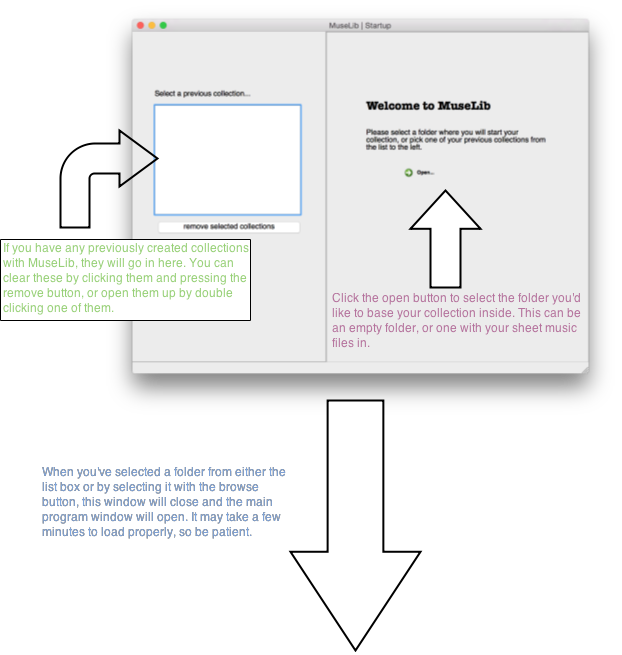
\includegraphics[width=400pt]{startup}
\caption{The window which will display on startup}
\label{fig:startup}	
\end{figure}

\subsection{Main view}
After the program has loaded, the main window shown in figure \ref{fig:main} will display. Panels to the left of this pane show a full listing of the files in your collection, which can be sorted by title, composer or lyricist, followed by a pane which displays any playlists you have created, followed by a third pane displaying playlists the system has generated for you. The auto generated playlists will automatically update with new pieces when you press the "refresh collection" option, located in the file menu.
\begin{figure}[H]
\centering
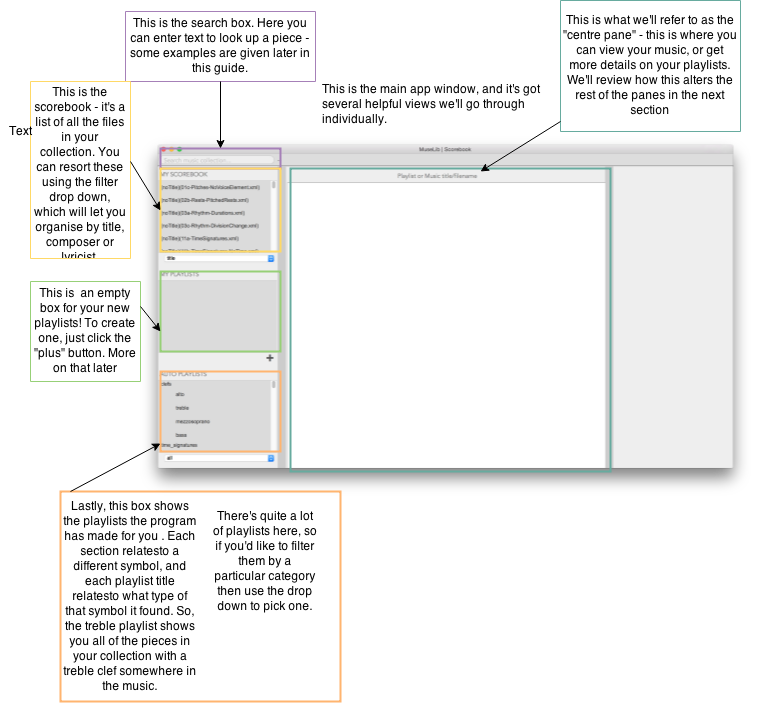
\includegraphics[width=500pt]{main_screenshot}
\caption{The window which will display on startup}
\label{fig:main}	
\end{figure}
\subsubsection{The User Created Playlist Widget}
The second widget from the top on the left is called the user created playlist widget. This will display all of the playlists you have created, as shown in figure \ref{fig:createdplaylists}. 
\begin{figure}[H]
\centering
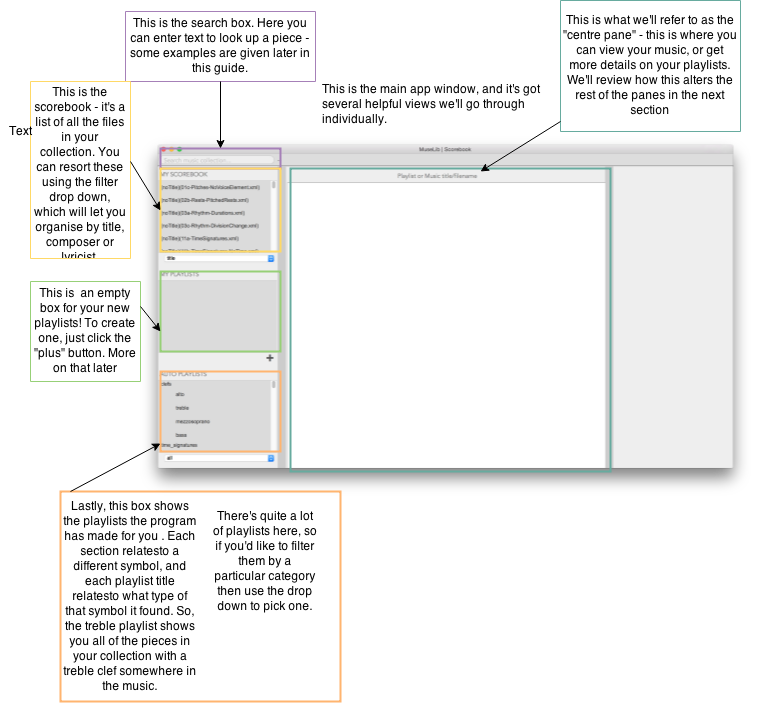
\includegraphics[width=500pt]{main_screenshot}
\caption{Window with playlists created by a user listed in second widget}
\label{fig:createdplaylists}	
\end{figure}

To add a new playlist to this list, press the add button, and a new popup will display as shown in figure \ref{fig:newplaylist}. Enter a title for this playlist, and search for pieces. The search functionality of this window is the same as the main window, as explained in section 2.3, so enter any information about the piece such as time signature, key etc in the same way you would in the main search box. These will be listed in the listbox below the text entry box, and can be reordered by dragging. Pieces can be removed from this list by selecting the item and pressing delete.
\begin{figure}[H]
\centering
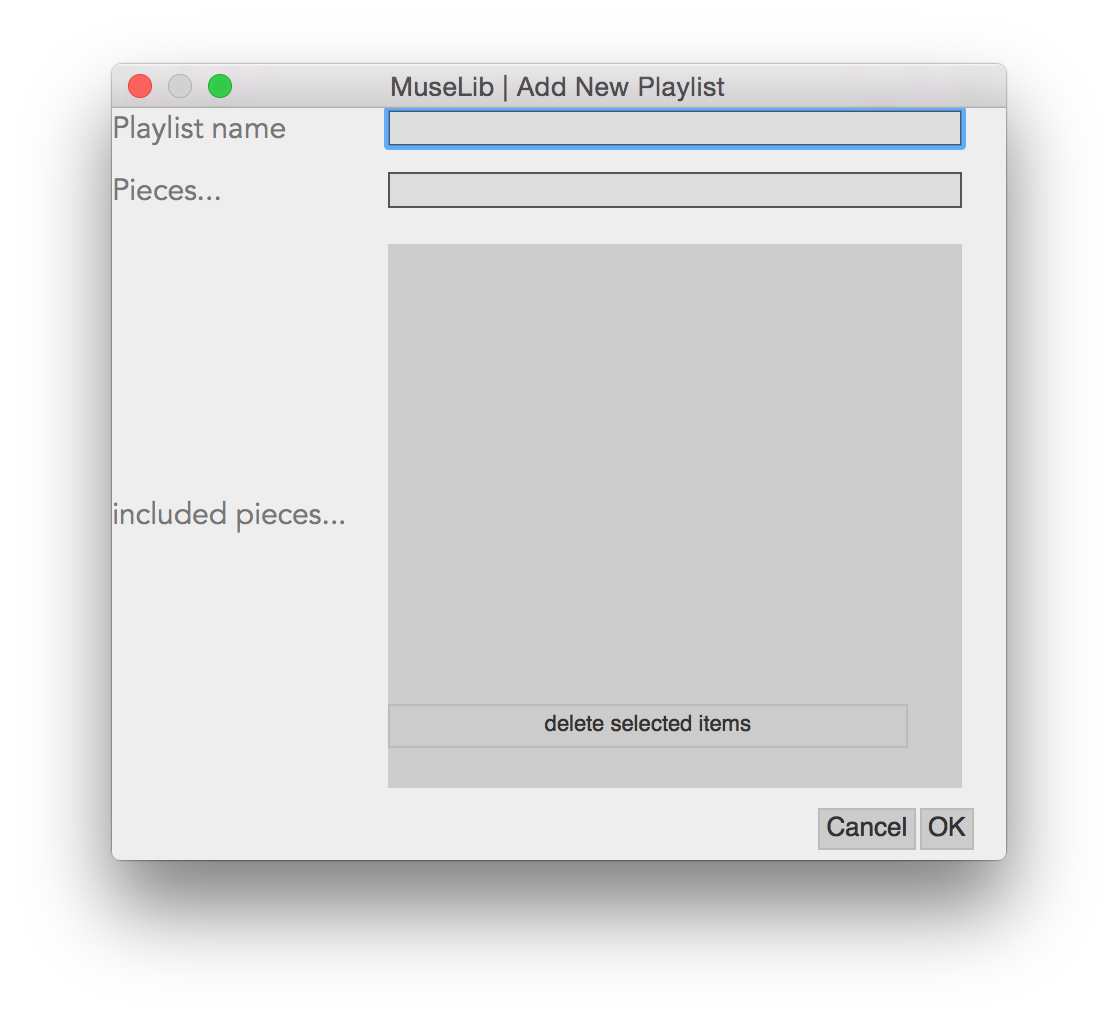
\includegraphics[width=\textwidth]{playlistpop}
\caption{Popup window for creating new playlists}
\label{fig:newplaylist}	
\end{figure}
Finally, press OK and the playlist will display in the widget to the left.

\subsection{Searching}
The search box at the top of the application allows you to browse your collection by entering information about the piece, as shown in figure \ref{fig:search}.
\begin{figure}[H]
\centering
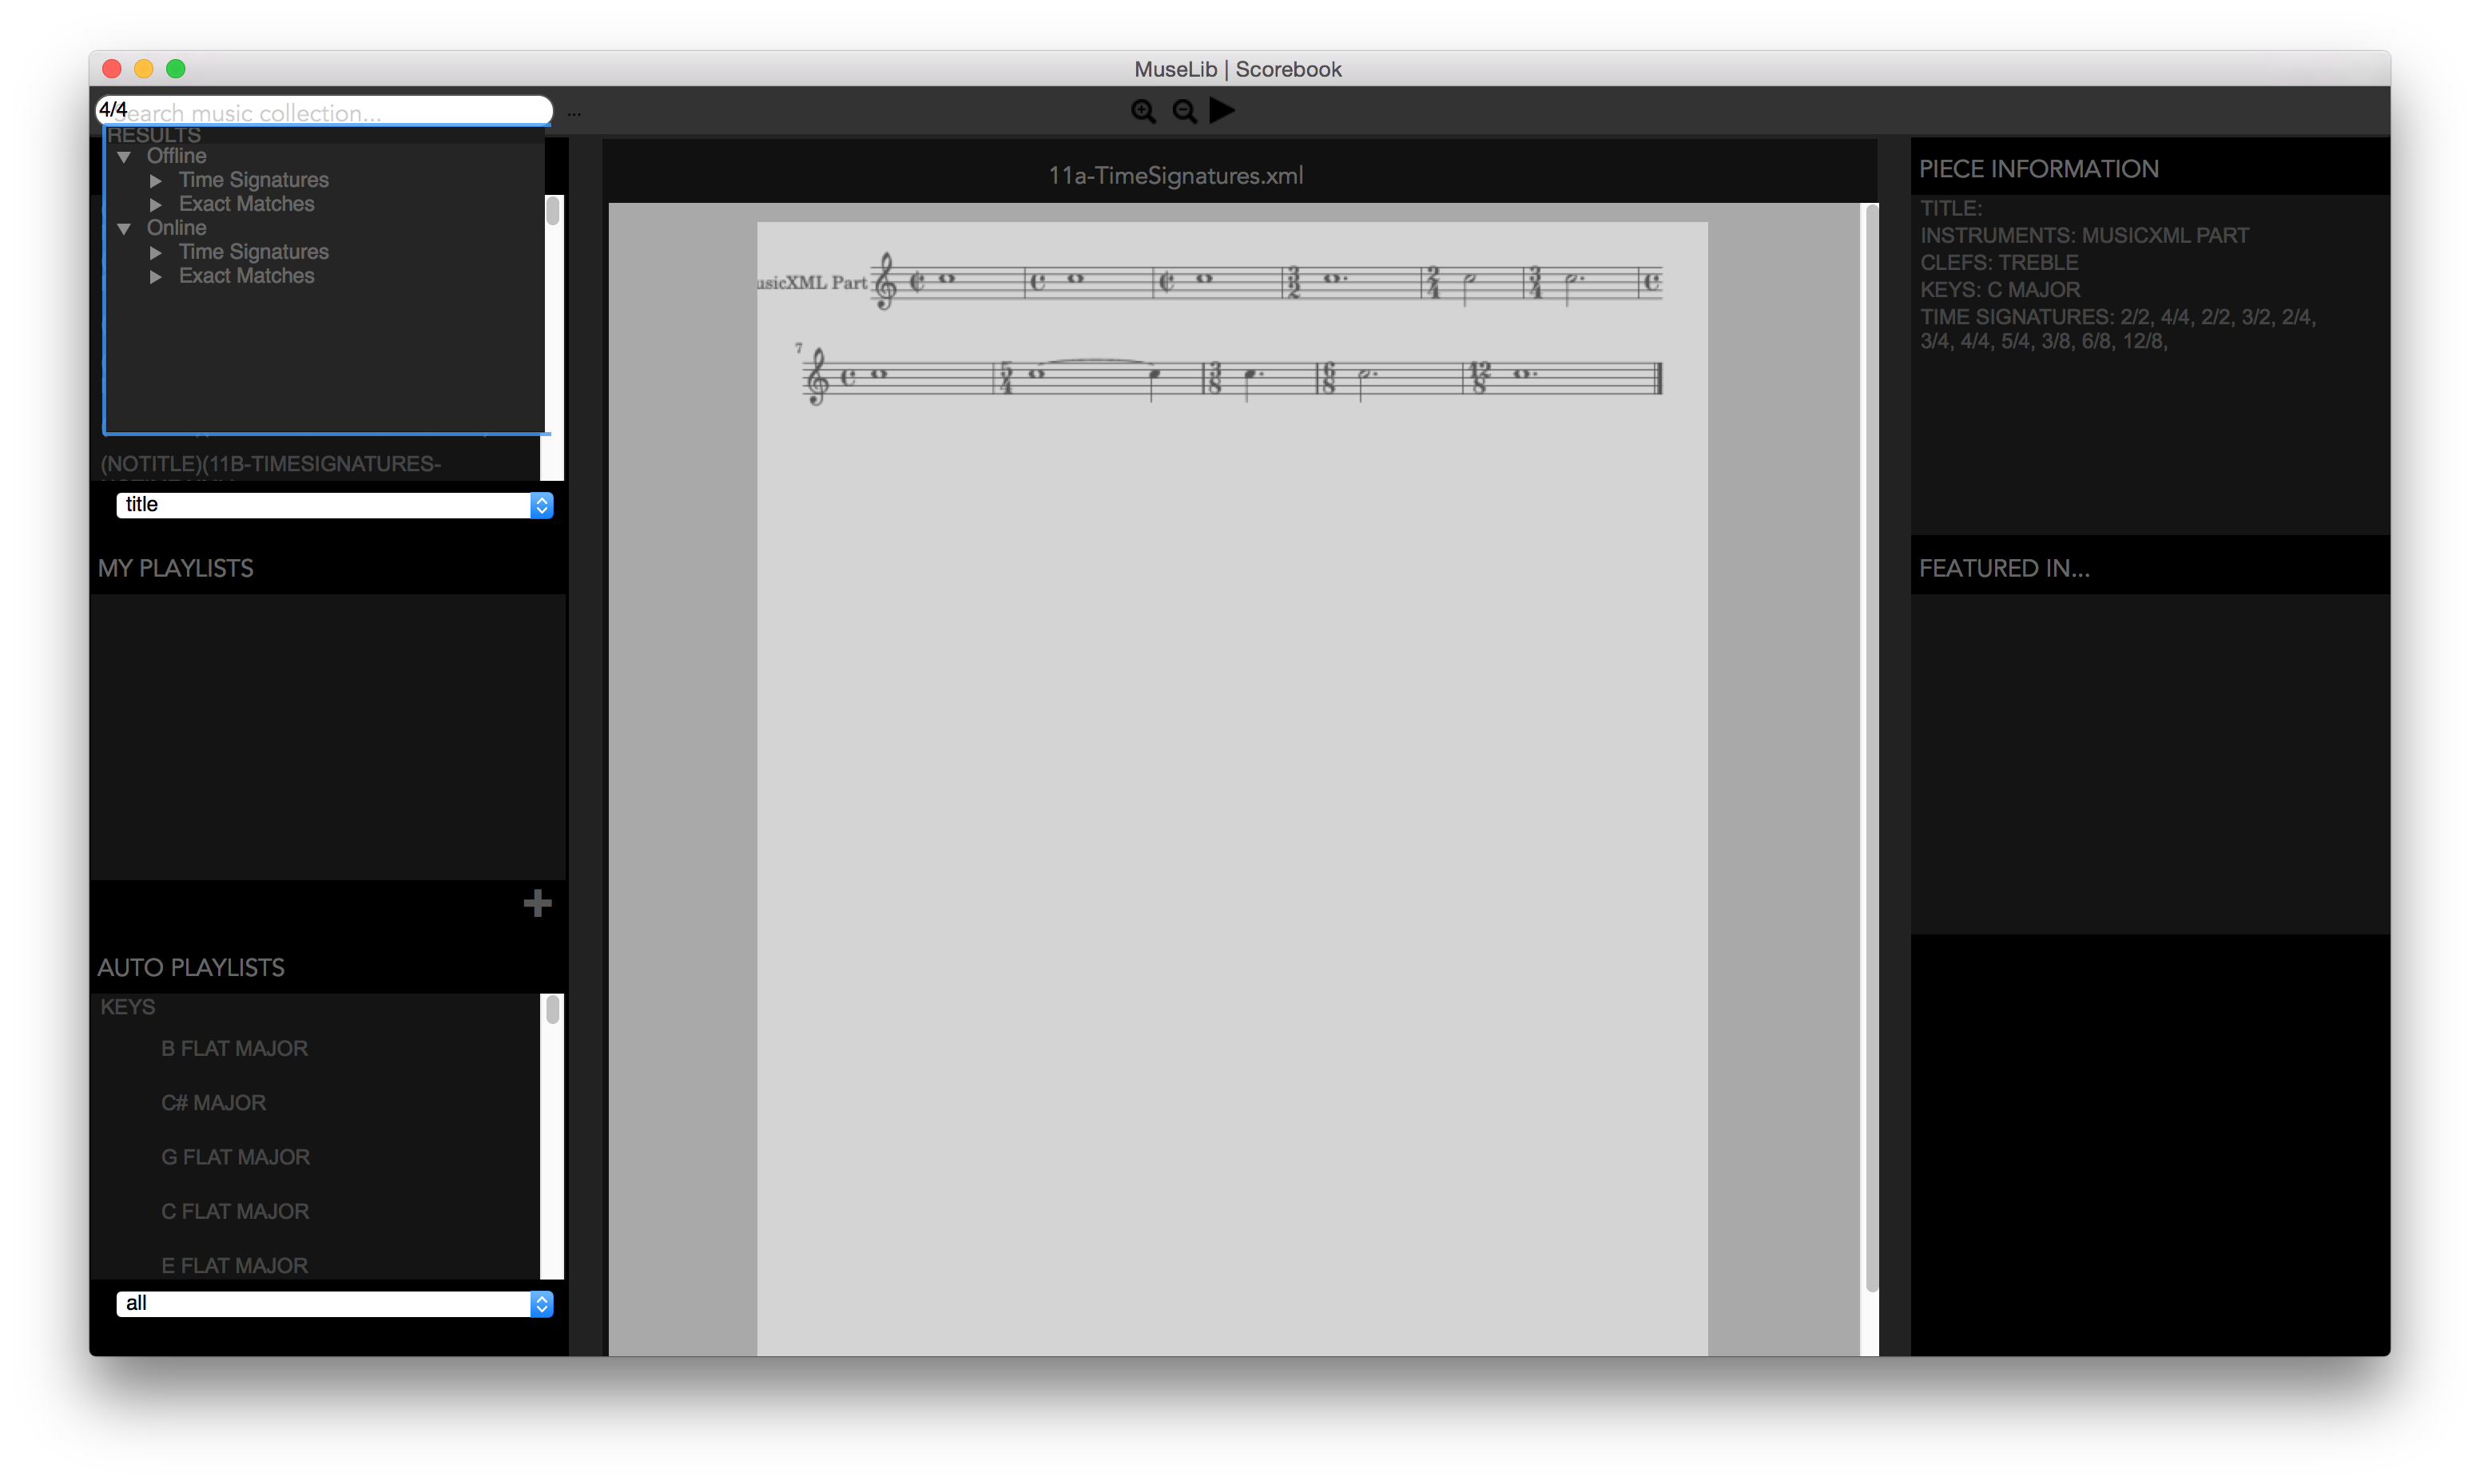
\includegraphics[width=500pt]{main_results}
\caption{Main window with search input results displaying}
\label{fig:search}	
\end{figure}

\subsubsection{Simple Searches}
In some instances, such as the query above, you may enter text into the box without needing to tell the system what you are looking for. Table \ref{table:commands} shows some of the commands you can use, separated by spaces.

\begin{table}[H]
\begin{tabu} to 1.05\textwidth {| X[l] | X[c] |} \hline
{Command} & {Result} \\ \hline
$<$letter$><$space$>$ followed by Major or Minor & System will look for pieces in this key (ignoring transposing instruments) \\ \hline
$<$number$>$/$<$number$>$ & System will search for a time signature \\ \hline
$<$rhythmicname$>$=$<$value$>$ & System will search for a tempo, where rhythmic name means quarter/crotchet, half/minim etc. \\ \hline
Text abc def & System will search individually for any pieces where the file name, title, composer, instrument names or lyricist match any of the individual words \\ \hline
"My name is fred" & System will search for the exact quote in all of the above \\ \hline
\end{tabu}
\caption{A table describing the command options for simple searches}
\label{table:commands}
\end{table}

\subsubsection{Complex Searches}
The structure laid out in section 2.3.1 manages to predict the majority of searches you might want to enter. However, some queries require more complexity, and as such "labels" are provided in order to achieve this. These are given in table \ref{table:commands_complex}.
\begin{table}[H]
\begin{tabu} to 1.05\textwidth {| X[l] | X[l] |} \hline
{\textbf{Command}} & {\textbf{Result}} \\ \hline
key:"C major" & System will look for pieces in this key \\ \hline
clef:treble & System will look for pieces with this clef in any part \\ \hline
meter:4/4 & System will search for a time signature \\ \hline
instrument:clarinet with:key:"C major" & System will search for pieces containing the instrument "clarinet" which is in the key of C major at some point in the piece \\ \hline
instrument:clarinet with:clef:bass & System will search for pieces containing the clarinet where the clarinet has a bass clef somewhere in the piece \\ \hline
instrument:clarinet with:clef:bass;key:"C major" & System will search for pieces containing the clarinet where the clarinet has a bass clef somewhere in the piece and is in C major somewhere in the piece \\ \hline
transposition:clarinet with:clef:bass;key:"C major" & System will search for pieces containing the clarinet, or if there is no clarinet, any instrument which has the same transposition \\ \hline
\end{tabu}
\caption{A table describing the command options for complex searches}
\label{table:commands_complex}
\end{table}

\subsubsection{Downloading new files}
When you search for files, the system will also provide you with suggestions which are located in online collections. You may choose to add these files to your collection simply by double clicking. This will open up a popup box as shown in figure \ref{fig:license}, which shows the license terms for that particular piece. When you click OK, the system will download and display the file.
\begin{figure}[H]
\centering
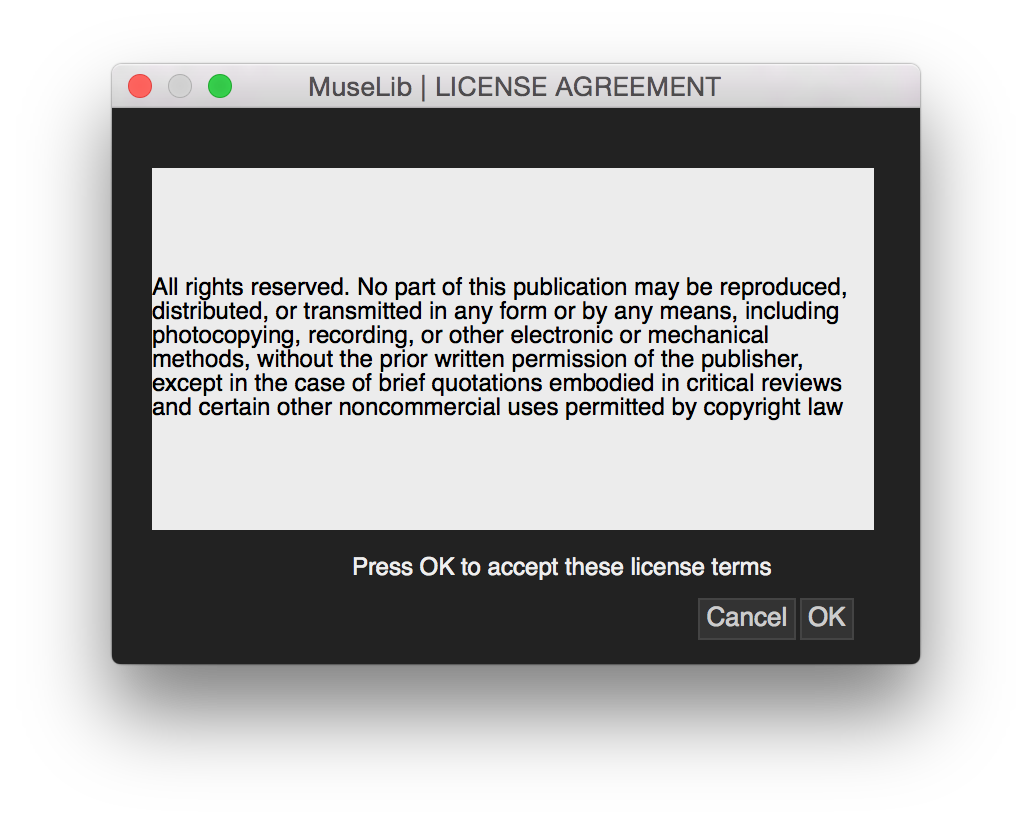
\includegraphics[width=400pt]{licensepop}
\caption{The popup which displays when a piece downloads}
\label{fig:license}	
\end{figure}

\subsection{Piece view}
When you view a piece, it will display in the middle portion and update the panes to the right according to data found, as shown in figure \ref{fig:piece}. The first pane to the right is for information about this piece. This displays all the information the system knows about the given piece.
The second pane displays any playlists you have created which feature this piece.
The third pane is a minimised version of the playlist browser. This will only display if you loaded this piece from the playlist view, as shown in figure \ref{fig:playlist}

\begin{figure}[H]
\centering
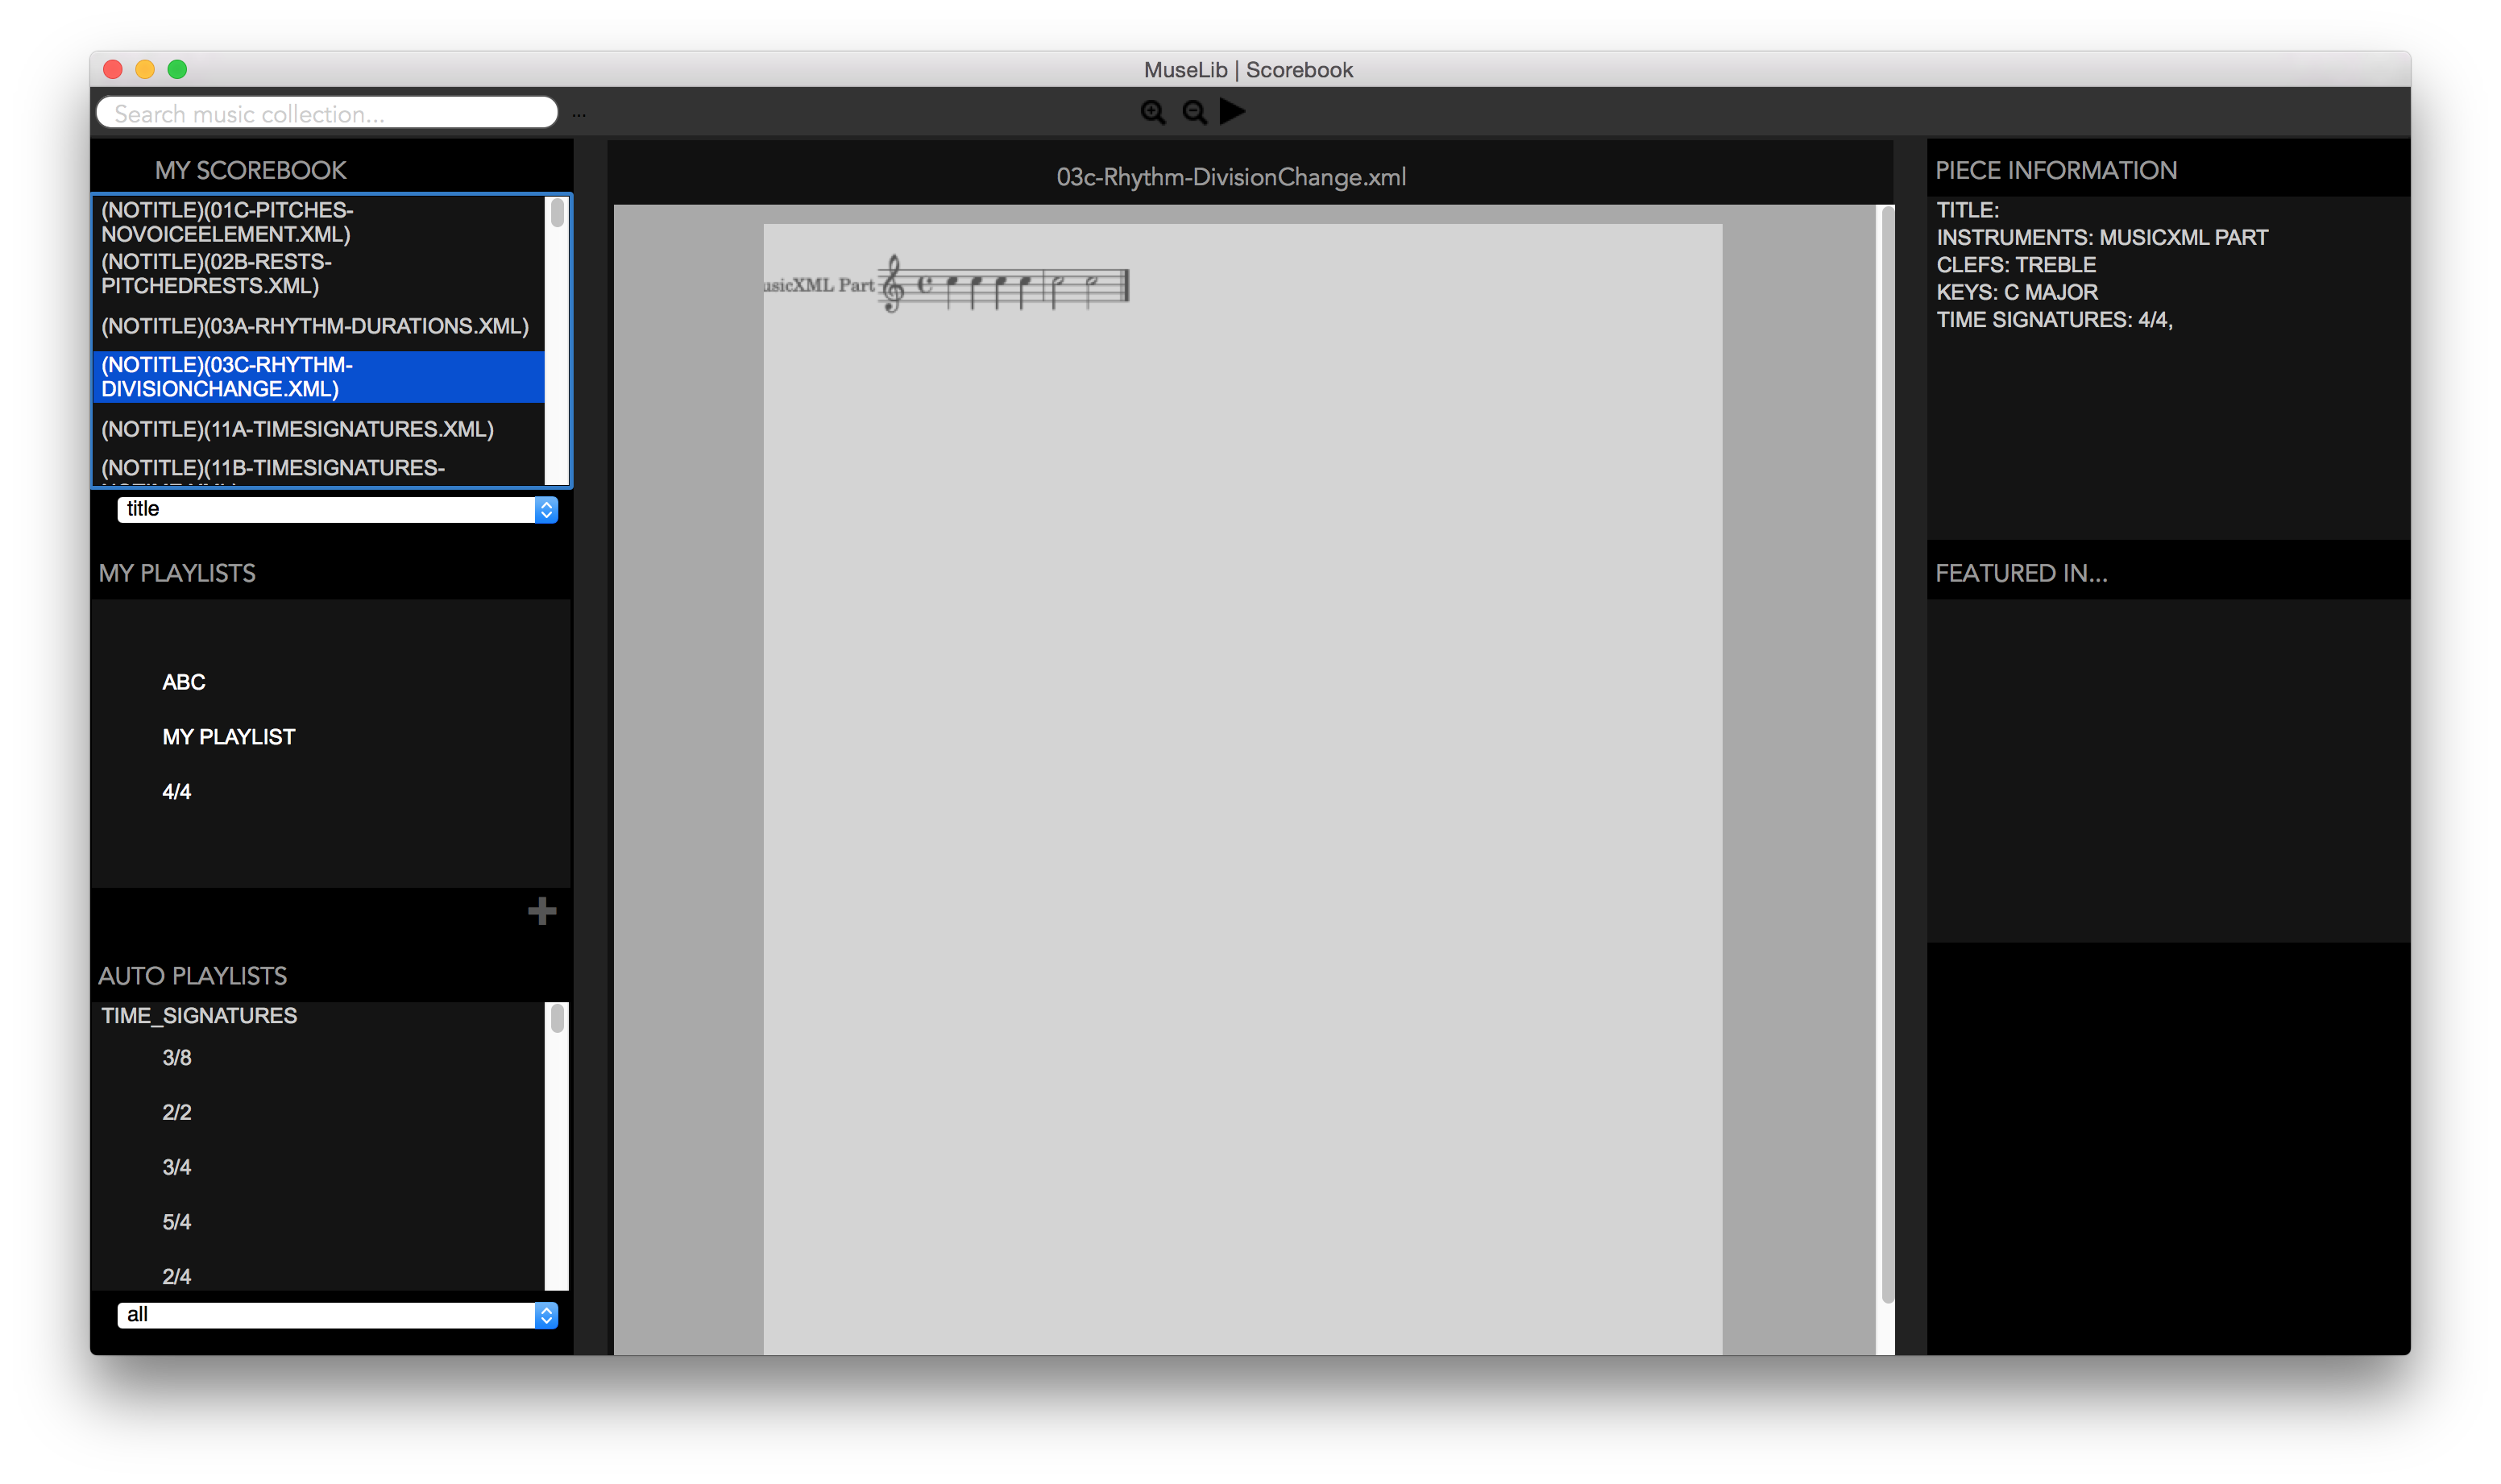
\includegraphics[width=500]{main_piece}
\caption{The main view showing a loaded piece}
\label{fig:piece}	
\end{figure}

There are also two buttons above the piece of music, the first of which allows you to zoom in, and the second zoom out. The third button is a feature which has yet to be put in.
\subsection{Playlist View}
When you select a playlist from either the user created widget or the auto generated playlists widget, the main window will update as shown in figure \ref{fig:playlist}. This displays a full list of pieces in the playlist together with all of the associated data.
\begin{figure}[H]
\centering
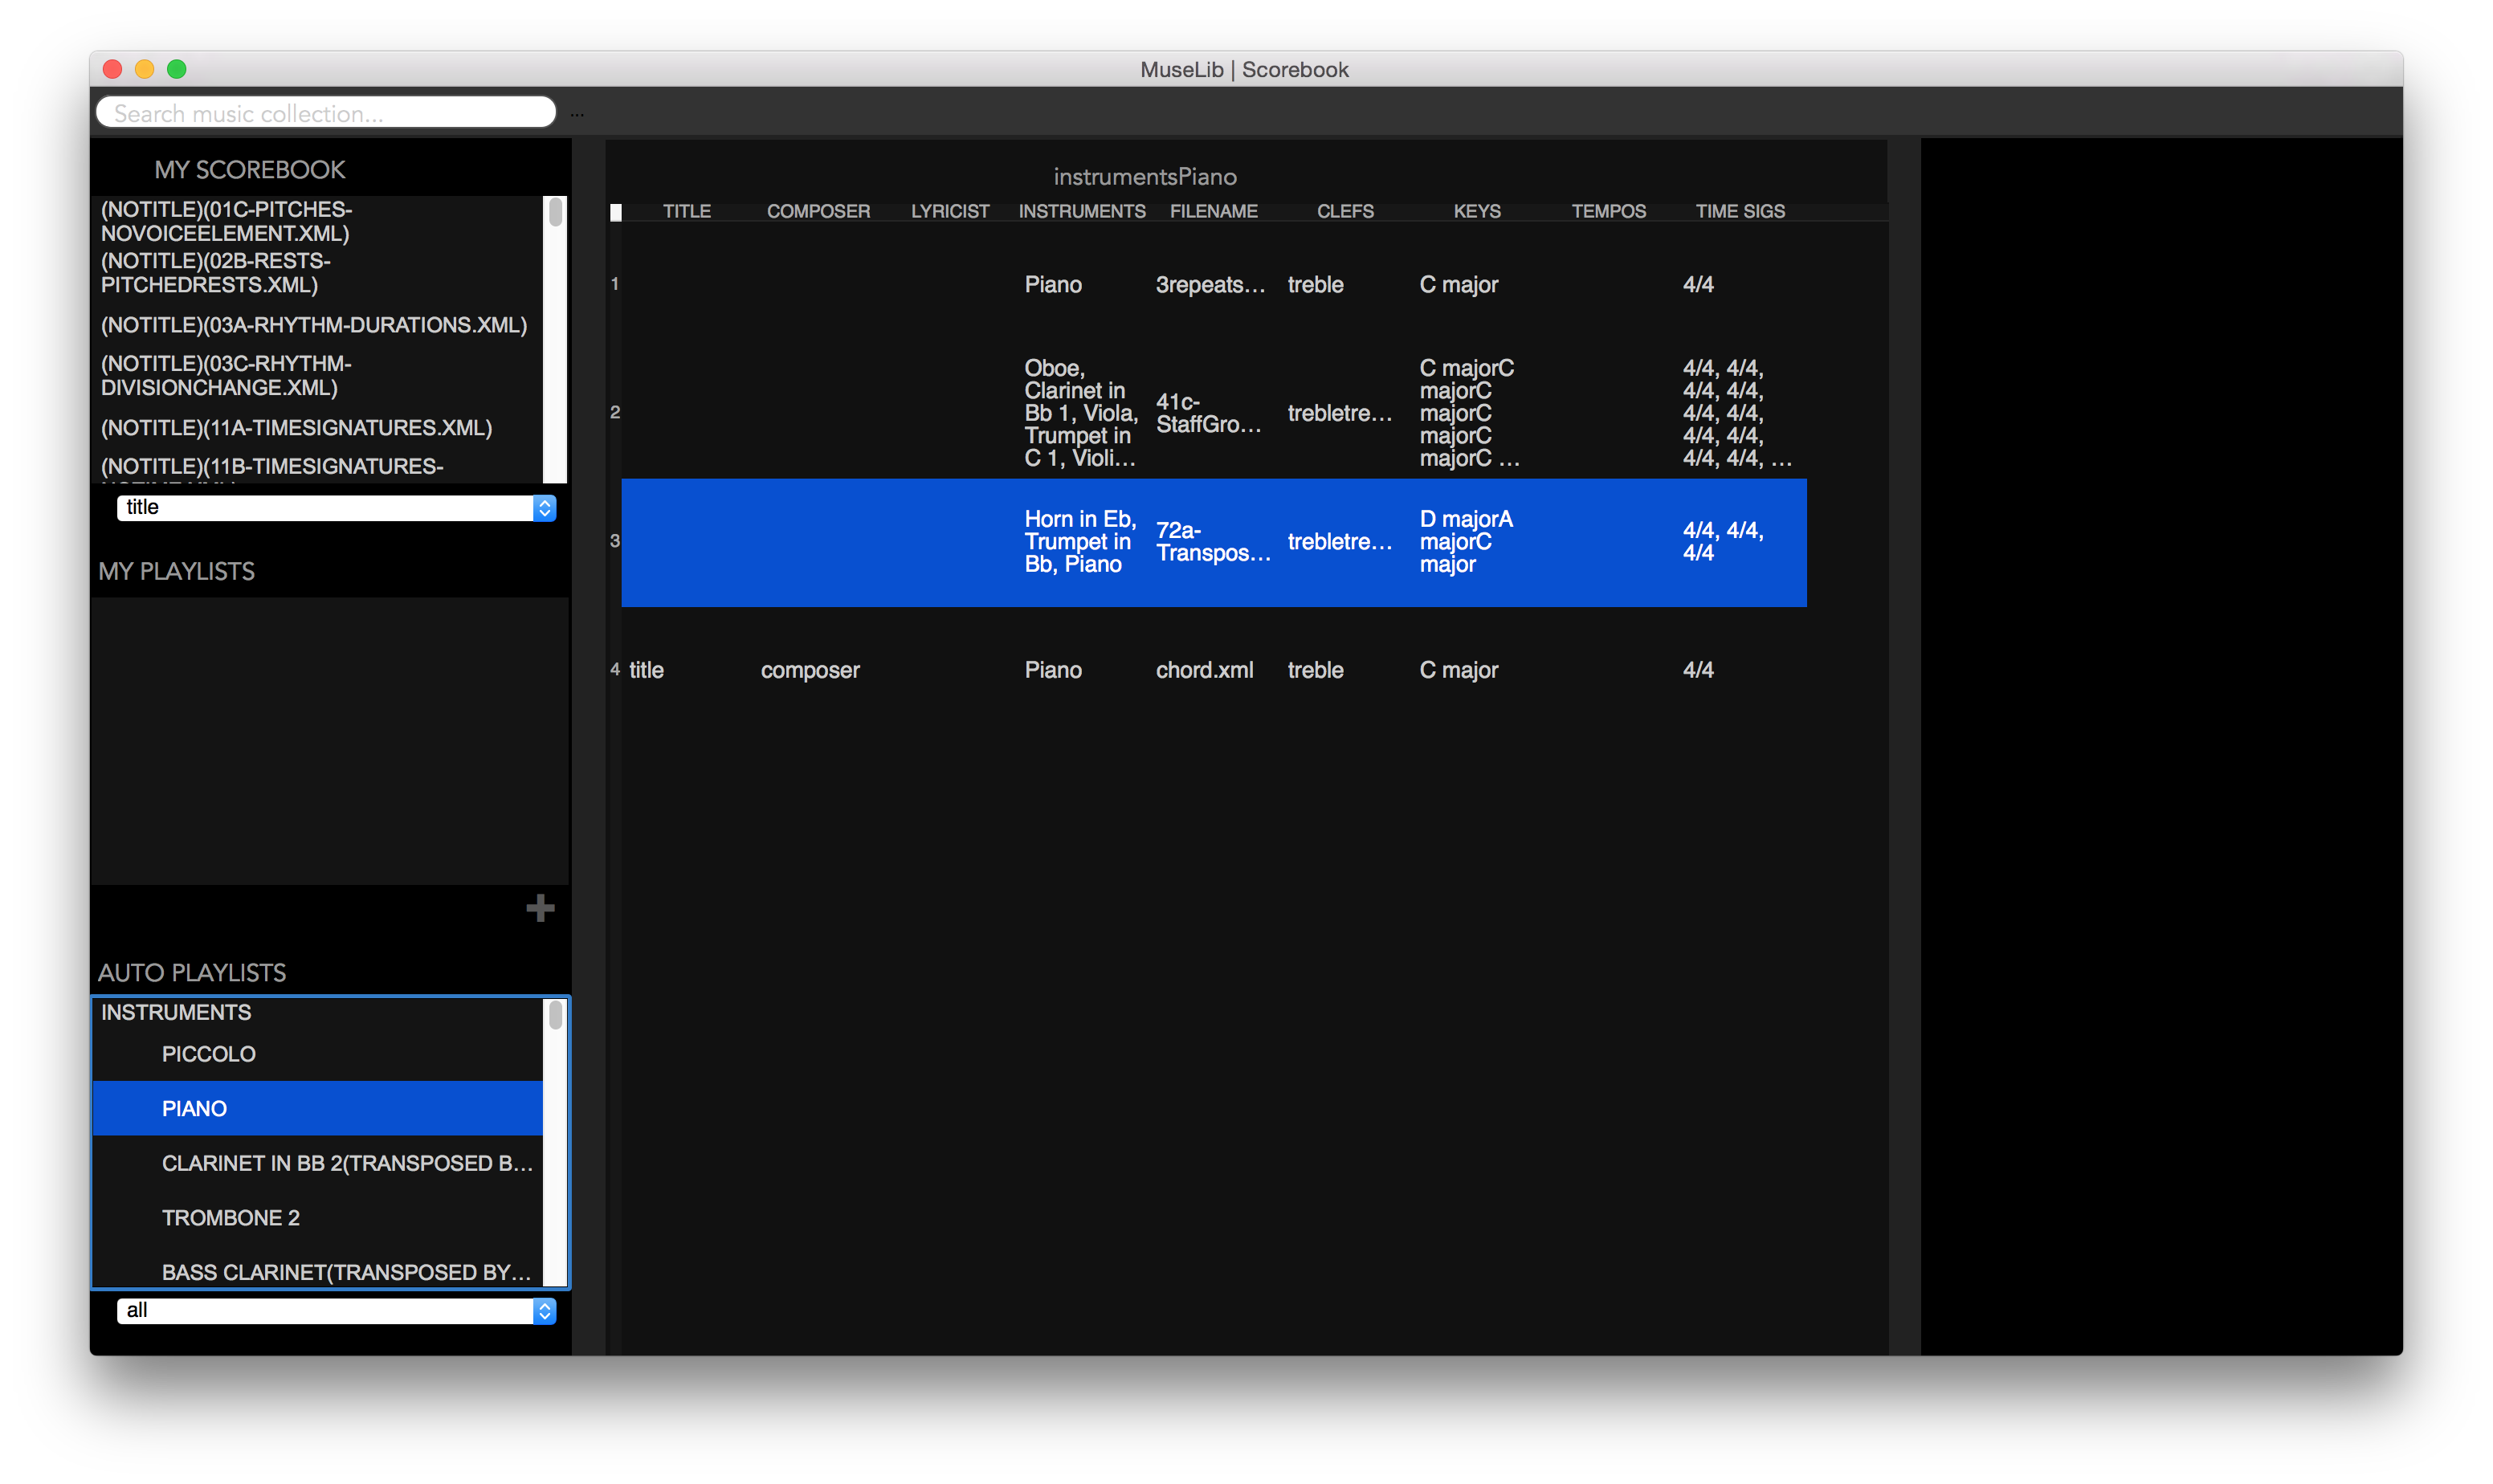
\includegraphics[width=500pt]{main_playlist}
\caption{The playlist view}
\label{fig:piece}	
\end{figure}

\subsubsection{Viewing a piece from the playlist view}
When you double click any of the pieces in a given playlist, the view will update as shown in figure \ref{fig:playlistbrowser}. A third widget has been displayed on the right, showing a full listing of the playlist. The widget has also highlighted the current piece you have selected.
\begin{figure}[H]
\centering
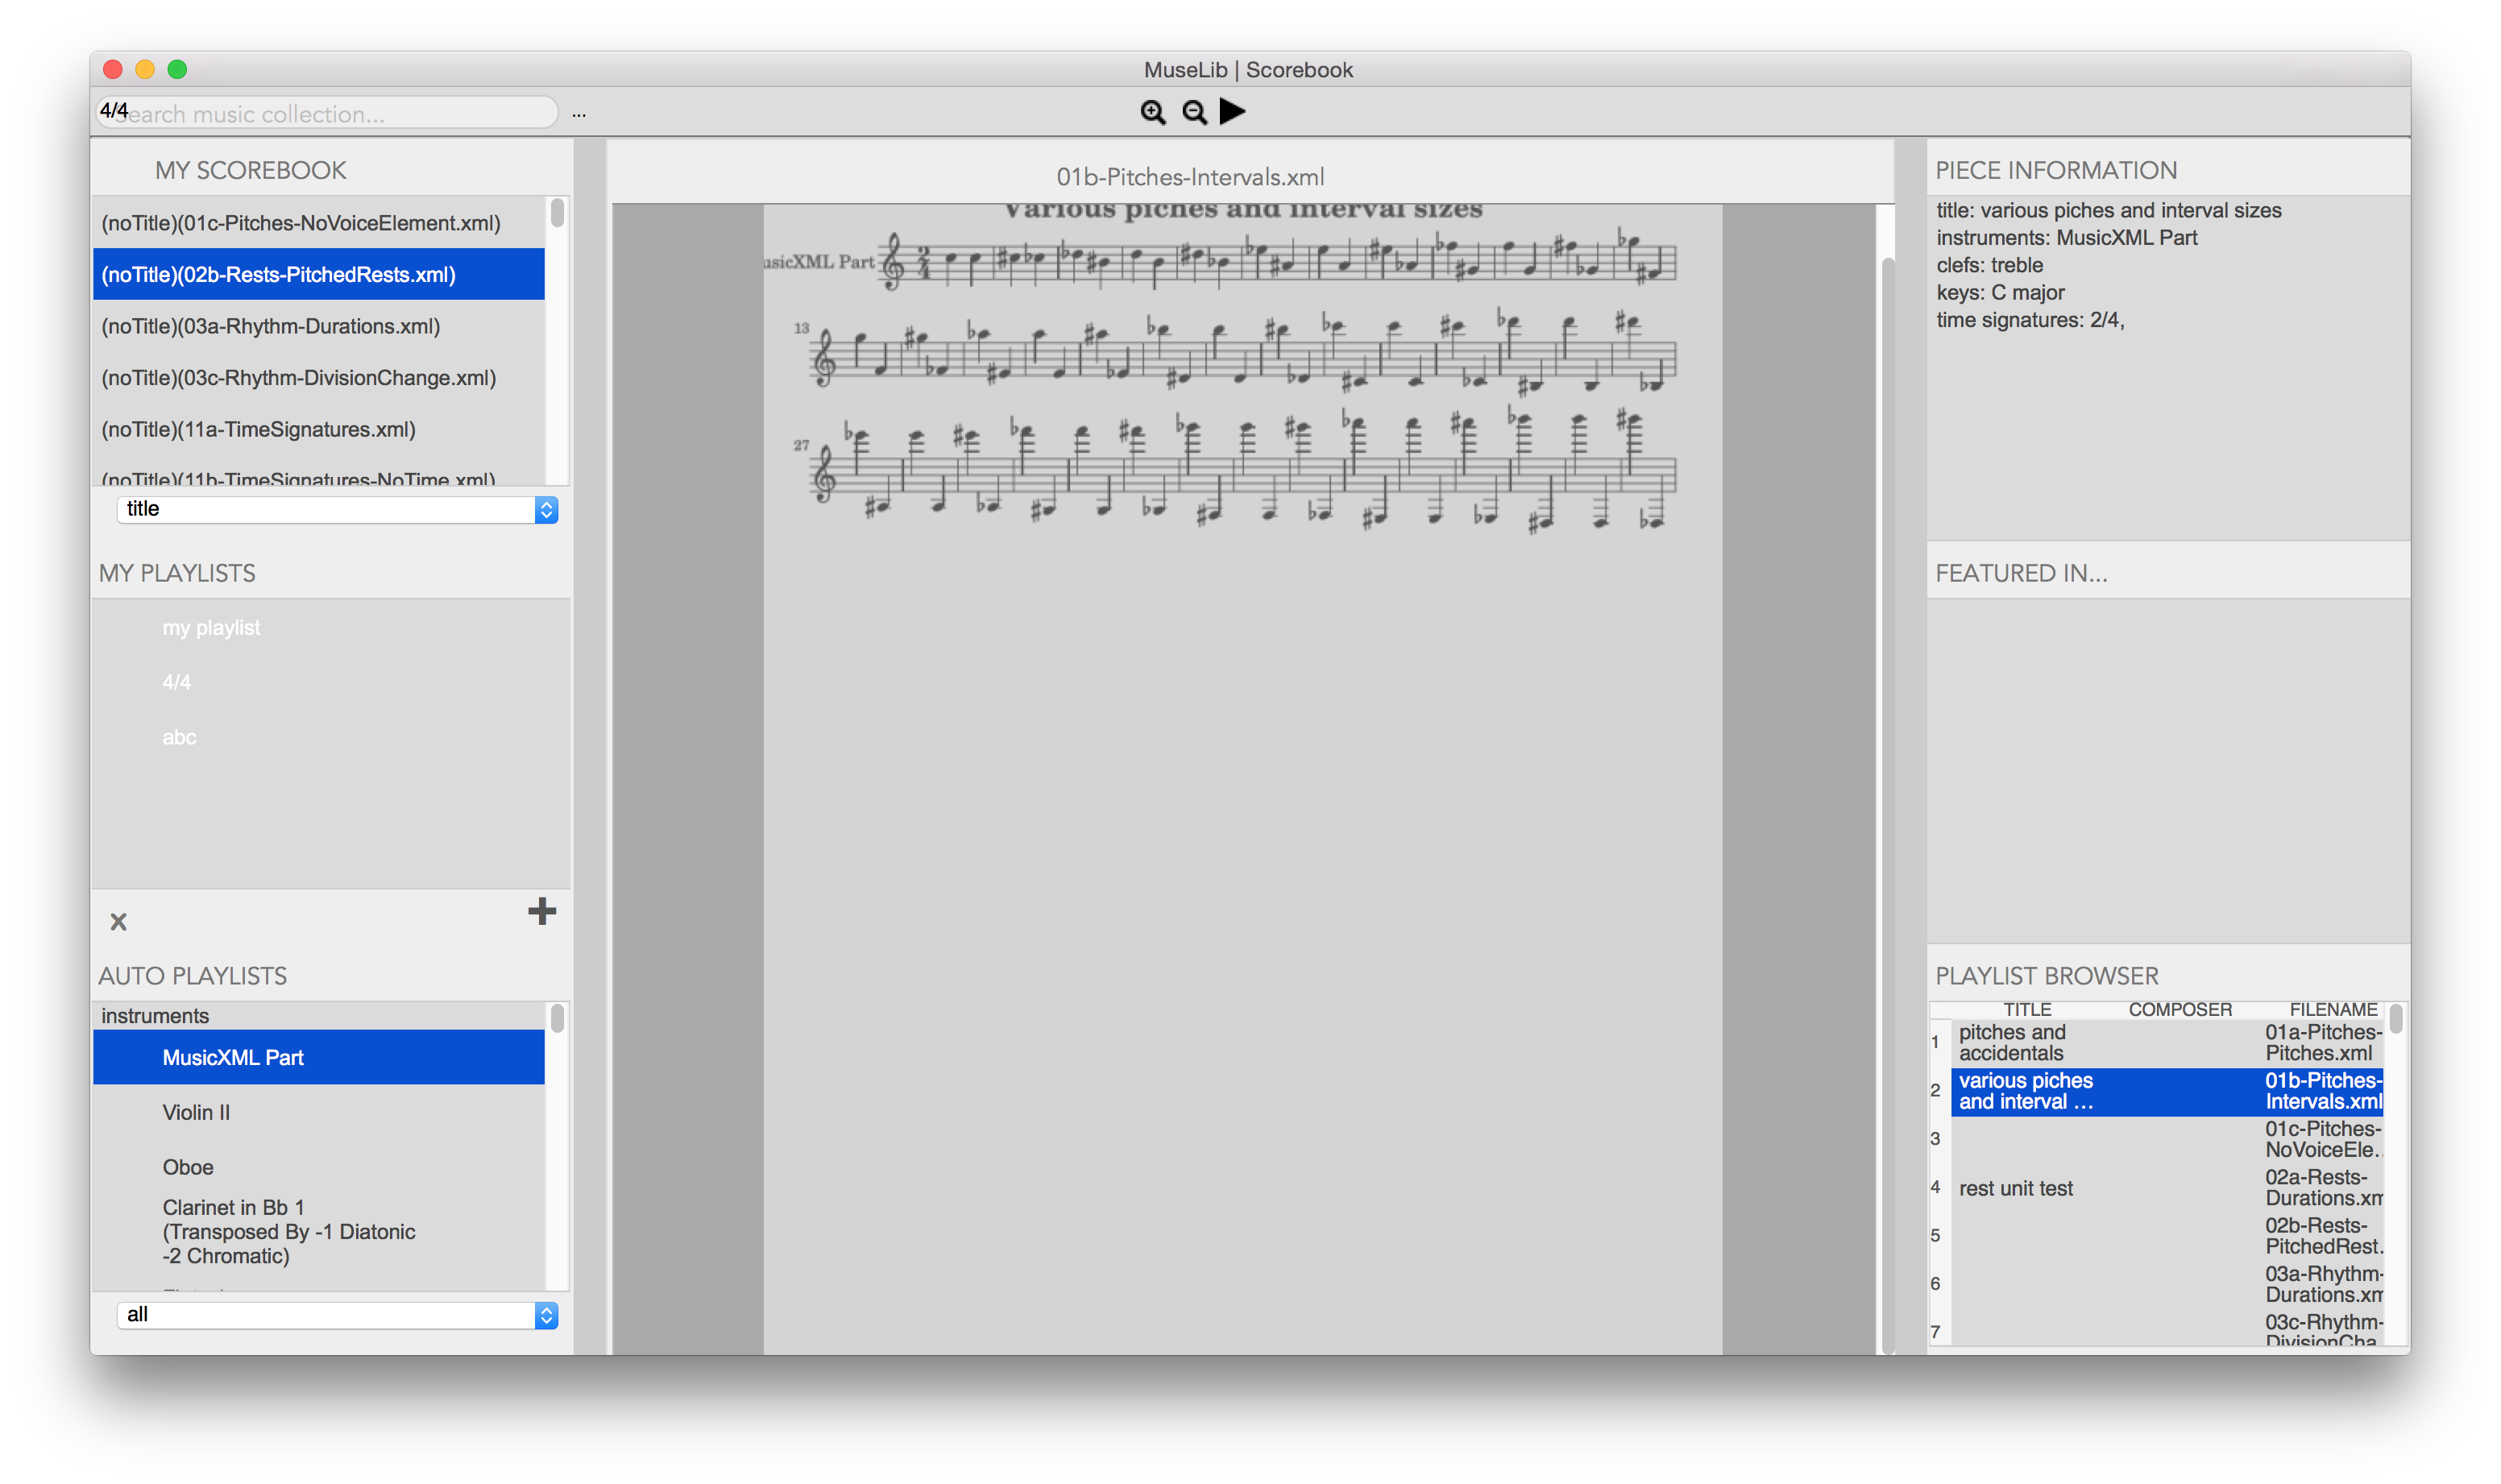
\includegraphics[width=500pt]{playlistbrowser}
\caption{The window which will display on startup}
\label{fig:playlistbrowser}	
\end{figure}

\subsection{Popups and Error Windows}
\subsubsection{The Import Popup}
If you wish to add a new file from inside the application which does not reside in the main collection folder, you may import it using the import window. To open it go to File->Import from the main window. The popup in figure \ref{fig:import} will display.
\begin{figure}[H]
\centering
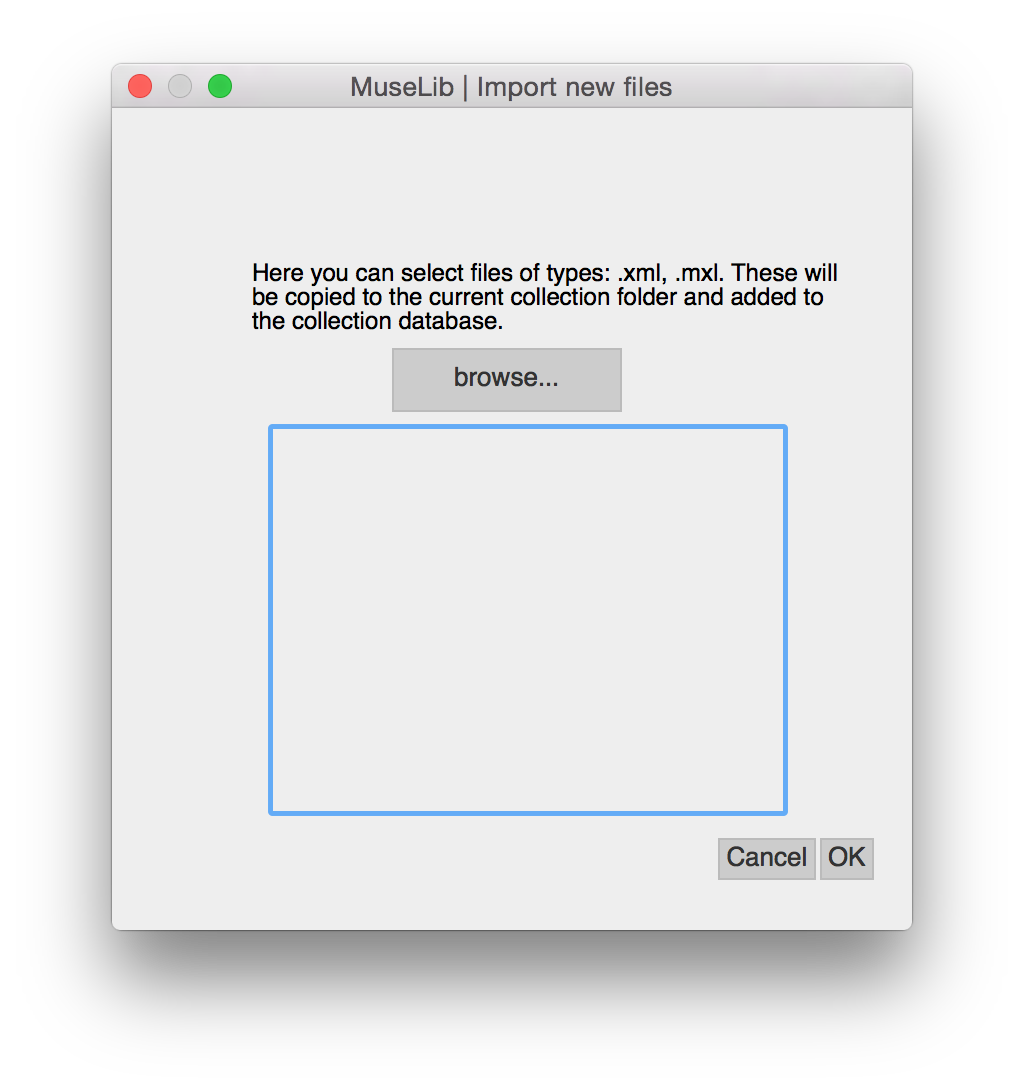
\includegraphics[width=500pt]{importpop}
\caption{The import popup window}
\label{fig:import}	
\end{figure}
Click browse to find the file. This window will allow you to select multiple files by browsing for one, selecting it and then browsing again. The list of files to copy will display in the listbox below the button.


\subsubsection{Error Popup}
Occasionally, files produce problems the system cannot handle - this includes drum tab and guitar tab. At other times there will be problems in the process the application could not process for different reasons, such as downloading files without internet connection. When these occur, the popup in figure \ref{fig:error} will display. If you find any odd errors, please report these to a developer.
\begin{figure}[H]
\centering
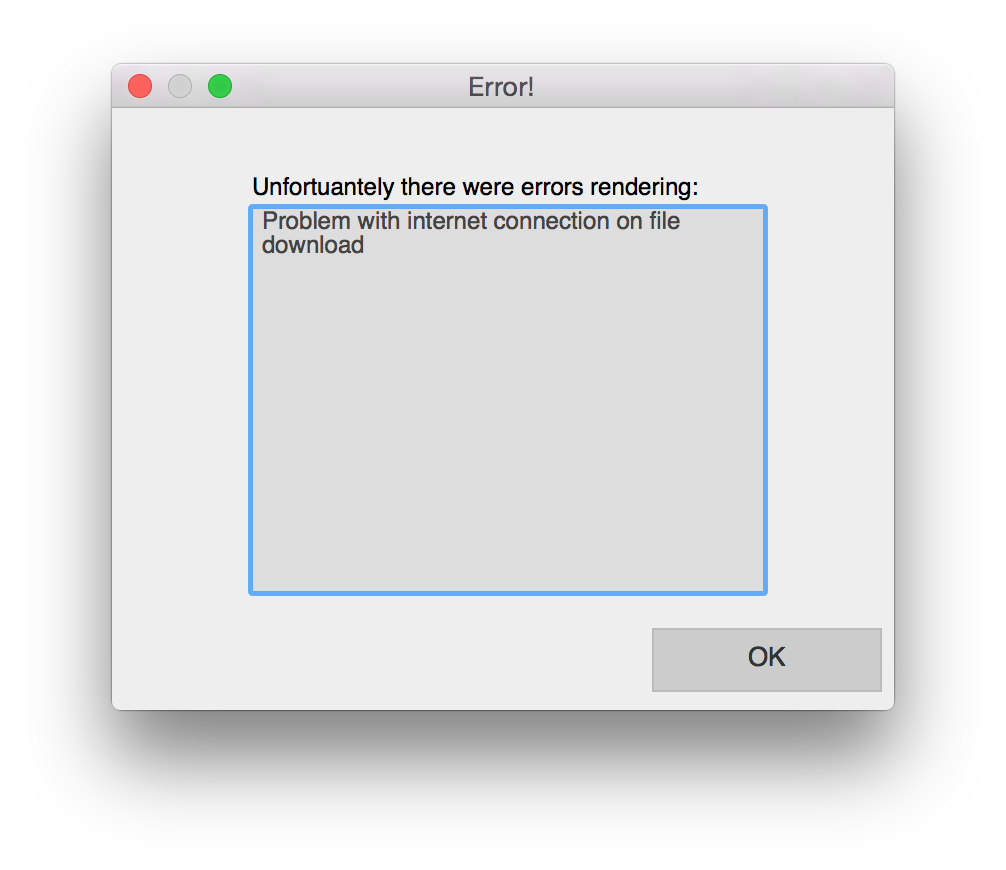
\includegraphics[width=500pt]{errorpop}
\caption{The window which will display on startup}
\label{fig:error}	
\end{figure}

\subsection{Customising your display}
\subsubsection{Themes}
The system comes with three different themes - the default which is light, dark and electric blue. These can be changed by clicking them in the theme menu as shown in figure \ref{fig:themes}. Their respective screenshots are shown in figures \ref{fig:theme1}, \ref{fig:theme2}, \ref{fig:theme3} and \ref{fig:theme4}.
\begin{figure}[H]
\centering
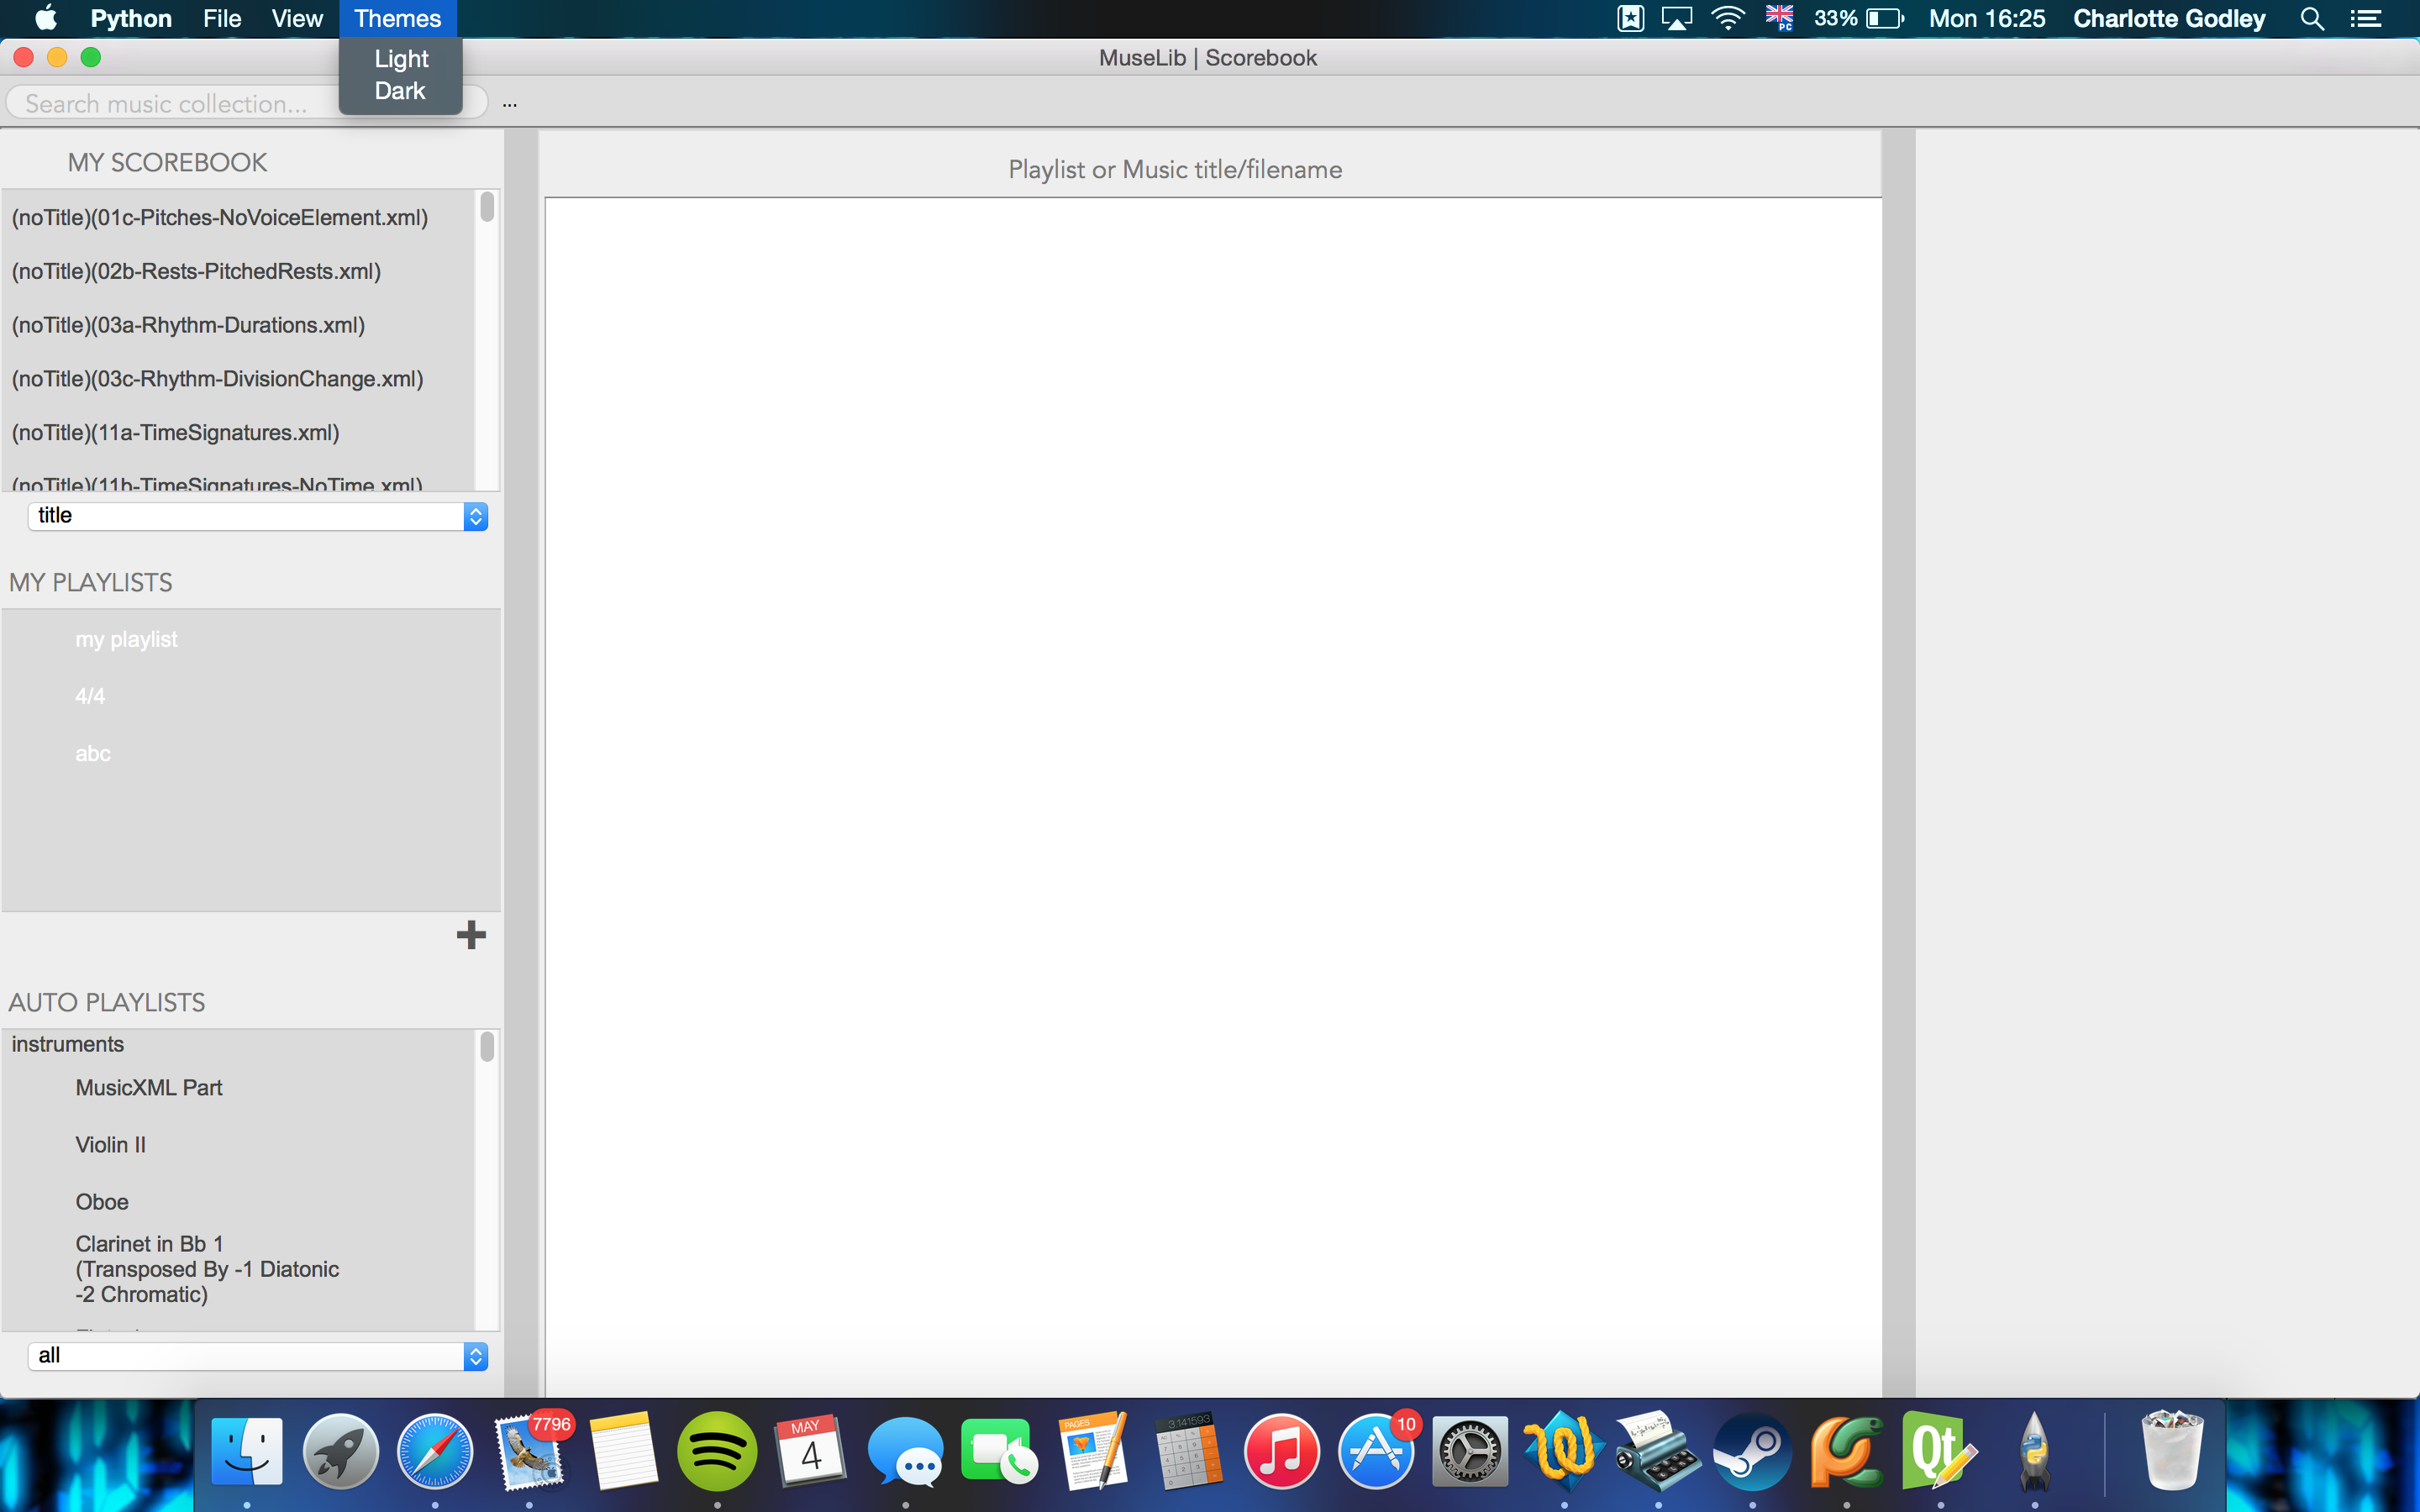
\includegraphics[width=500pt]{theme}
\caption{The themes menu}
\label{fig:themes}	
\end{figure}

\begin{figure}[H]
\centering
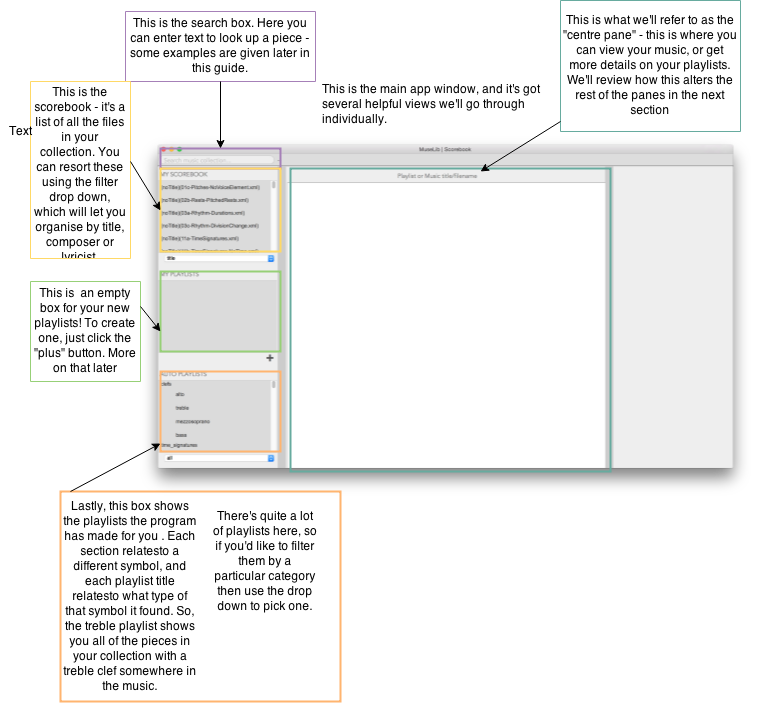
\includegraphics[width=400pt]{main_screenshot}
\caption{The light theme}
\label{fig:theme1}	
\end{figure}

\begin{figure}[H]
\centering
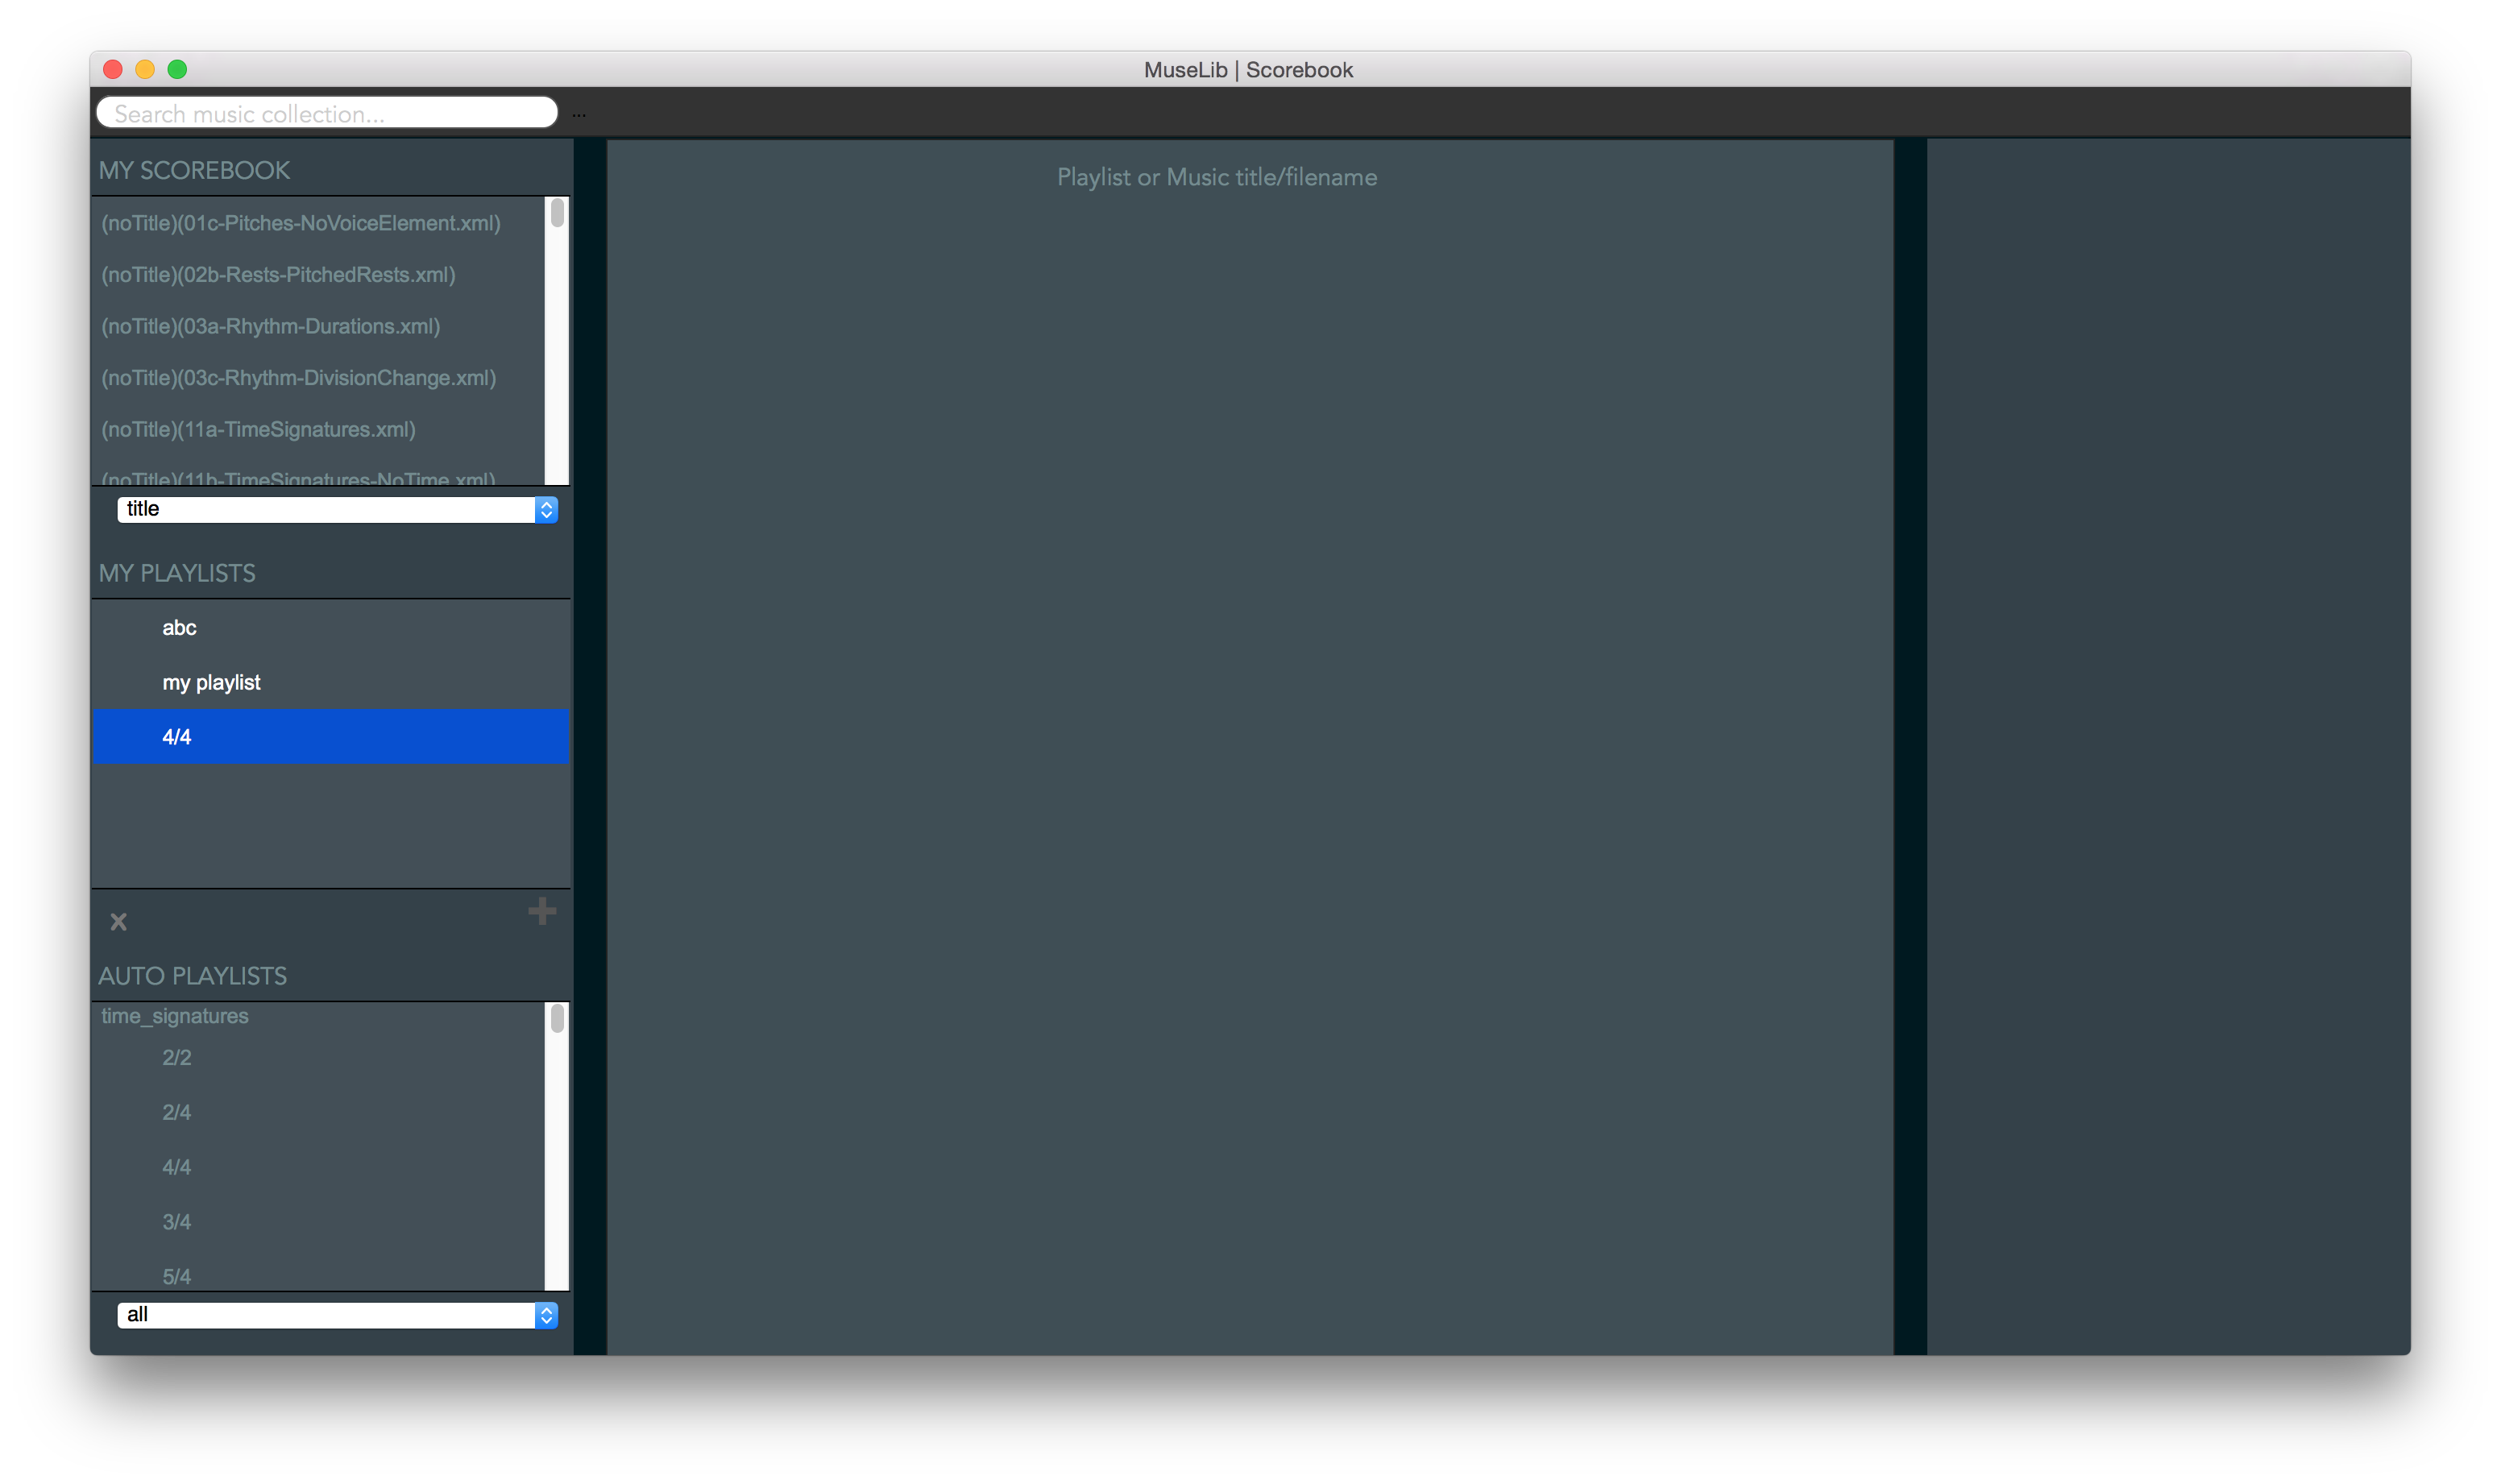
\includegraphics[width=400pt]{main_dark}
\caption{The dark theme}
\label{fig:theme2}	
\end{figure}

\begin{figure}[H]
\centering
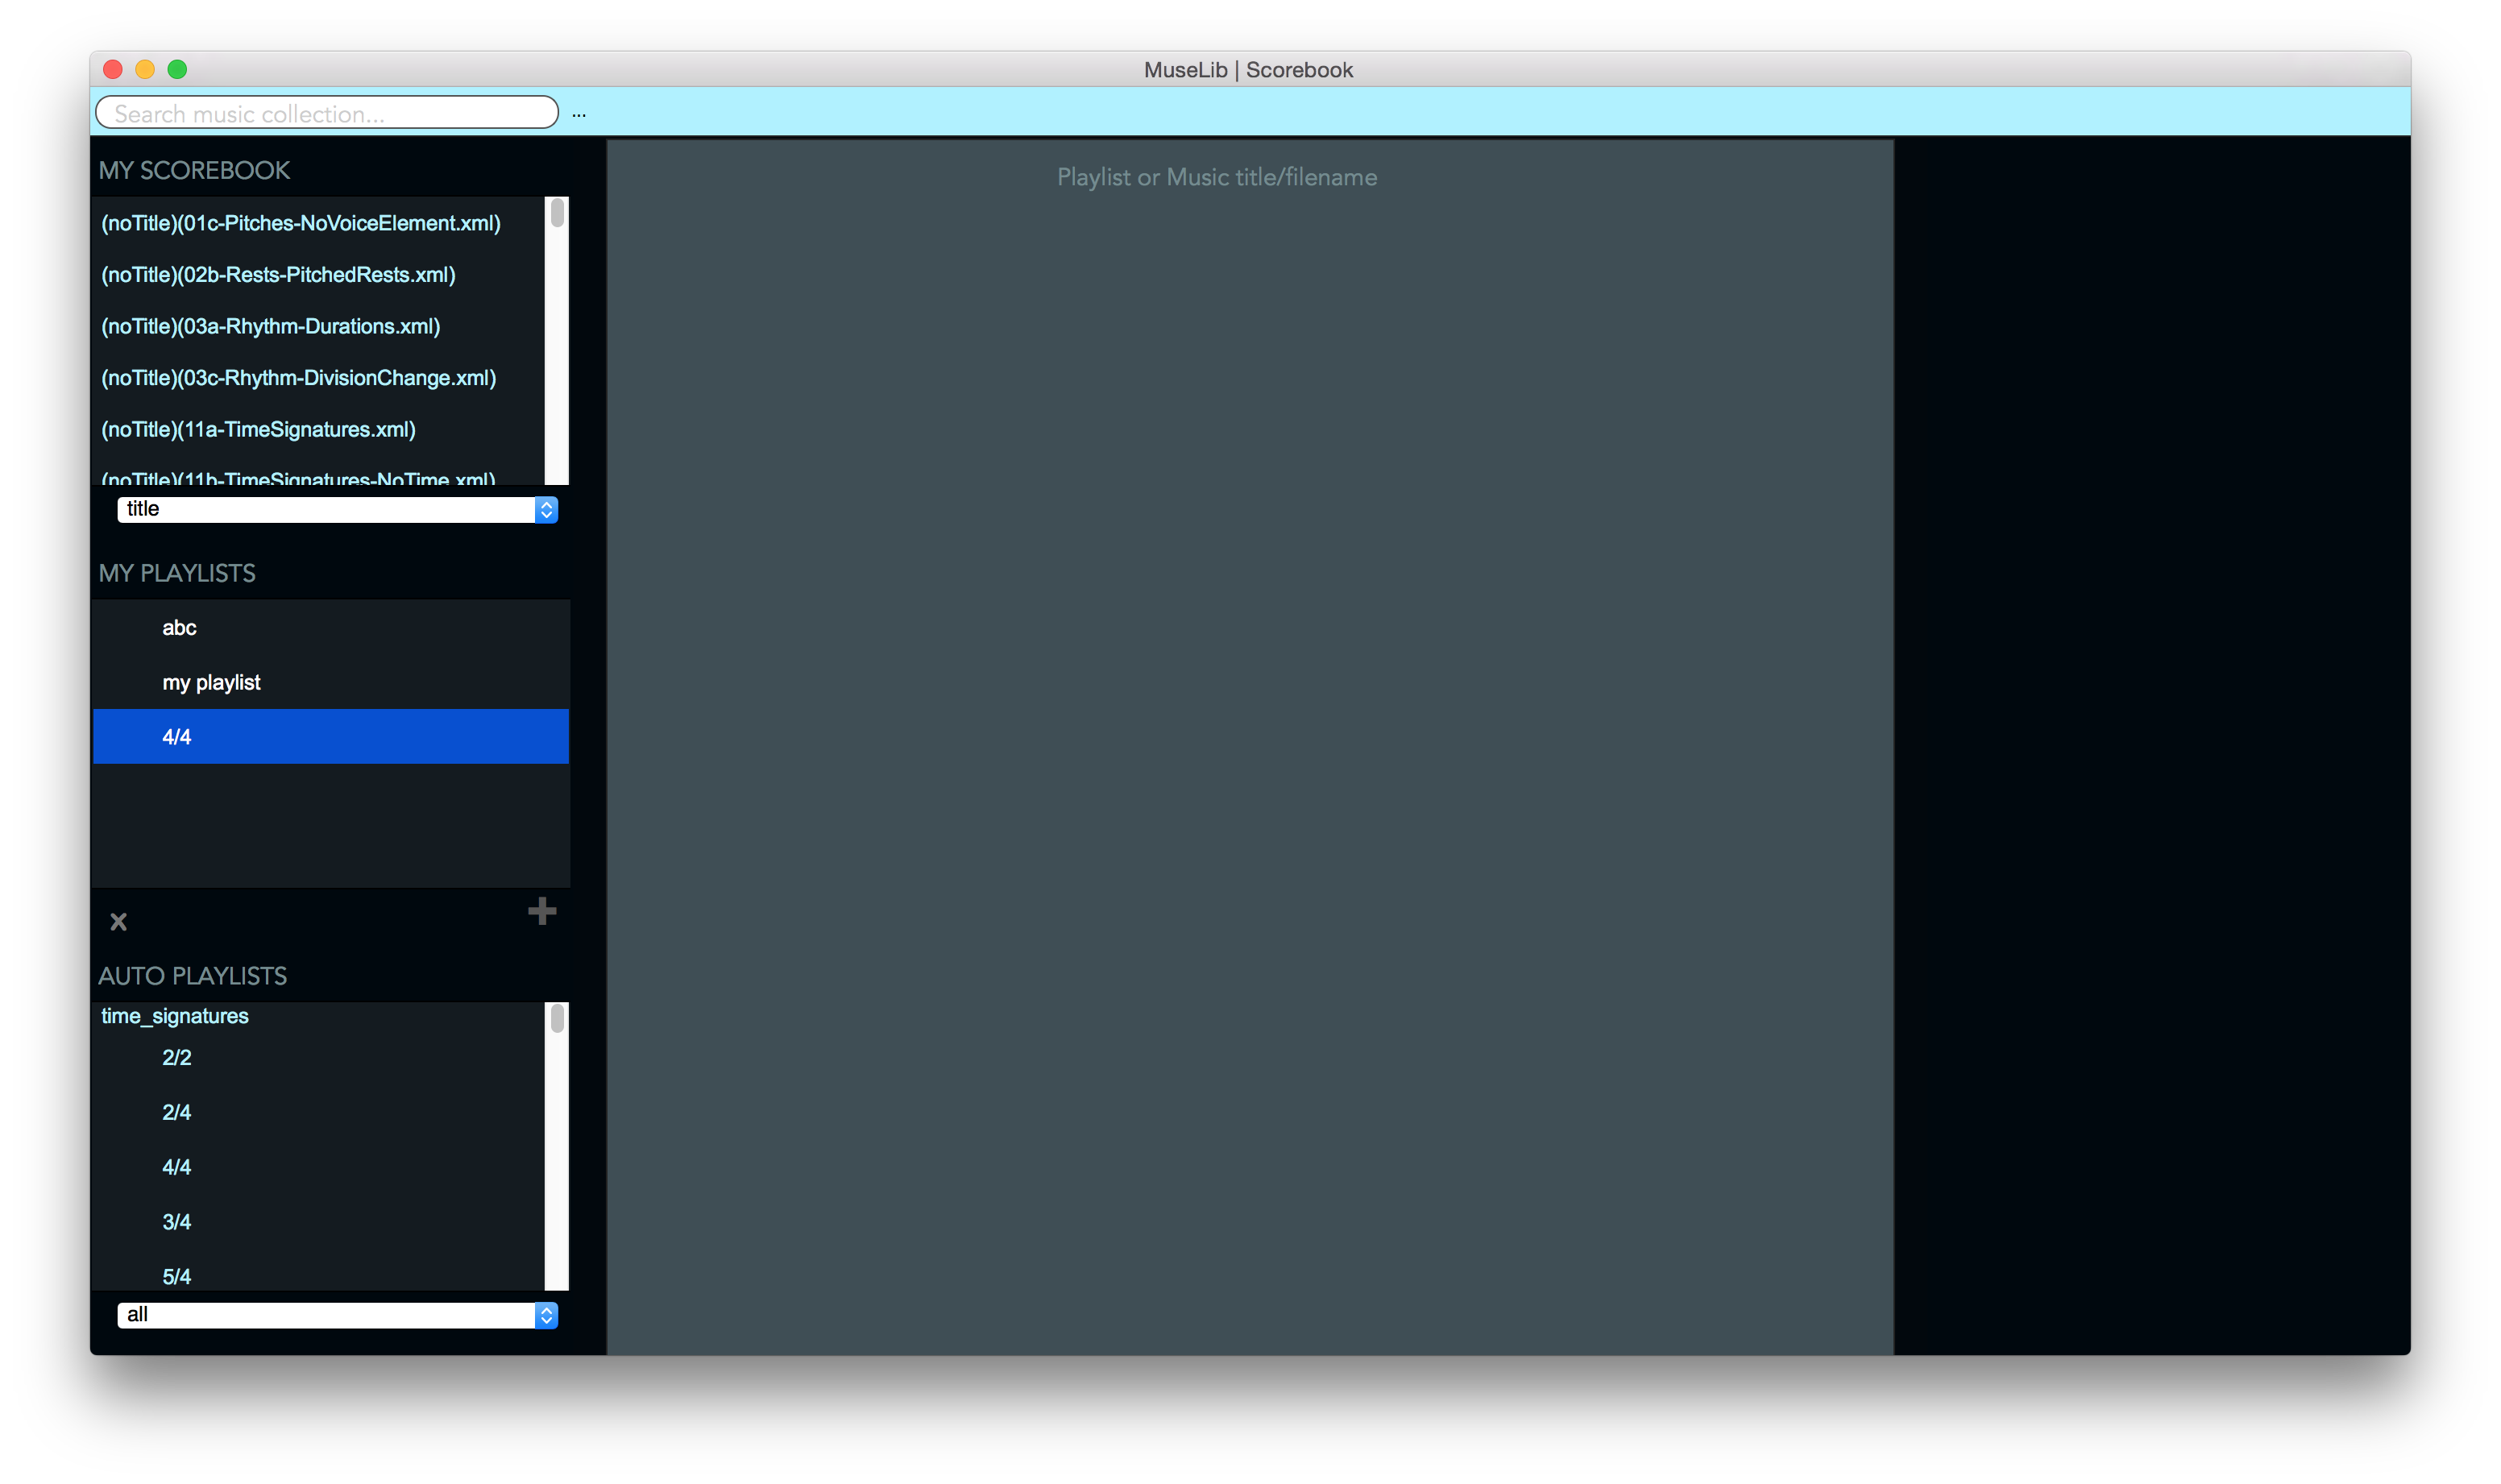
\includegraphics[width=400pt]{main_electric}
\caption{The electric blue theme}
\label{fig:theme3}	
\end{figure}

\begin{figure}[H]
\centering
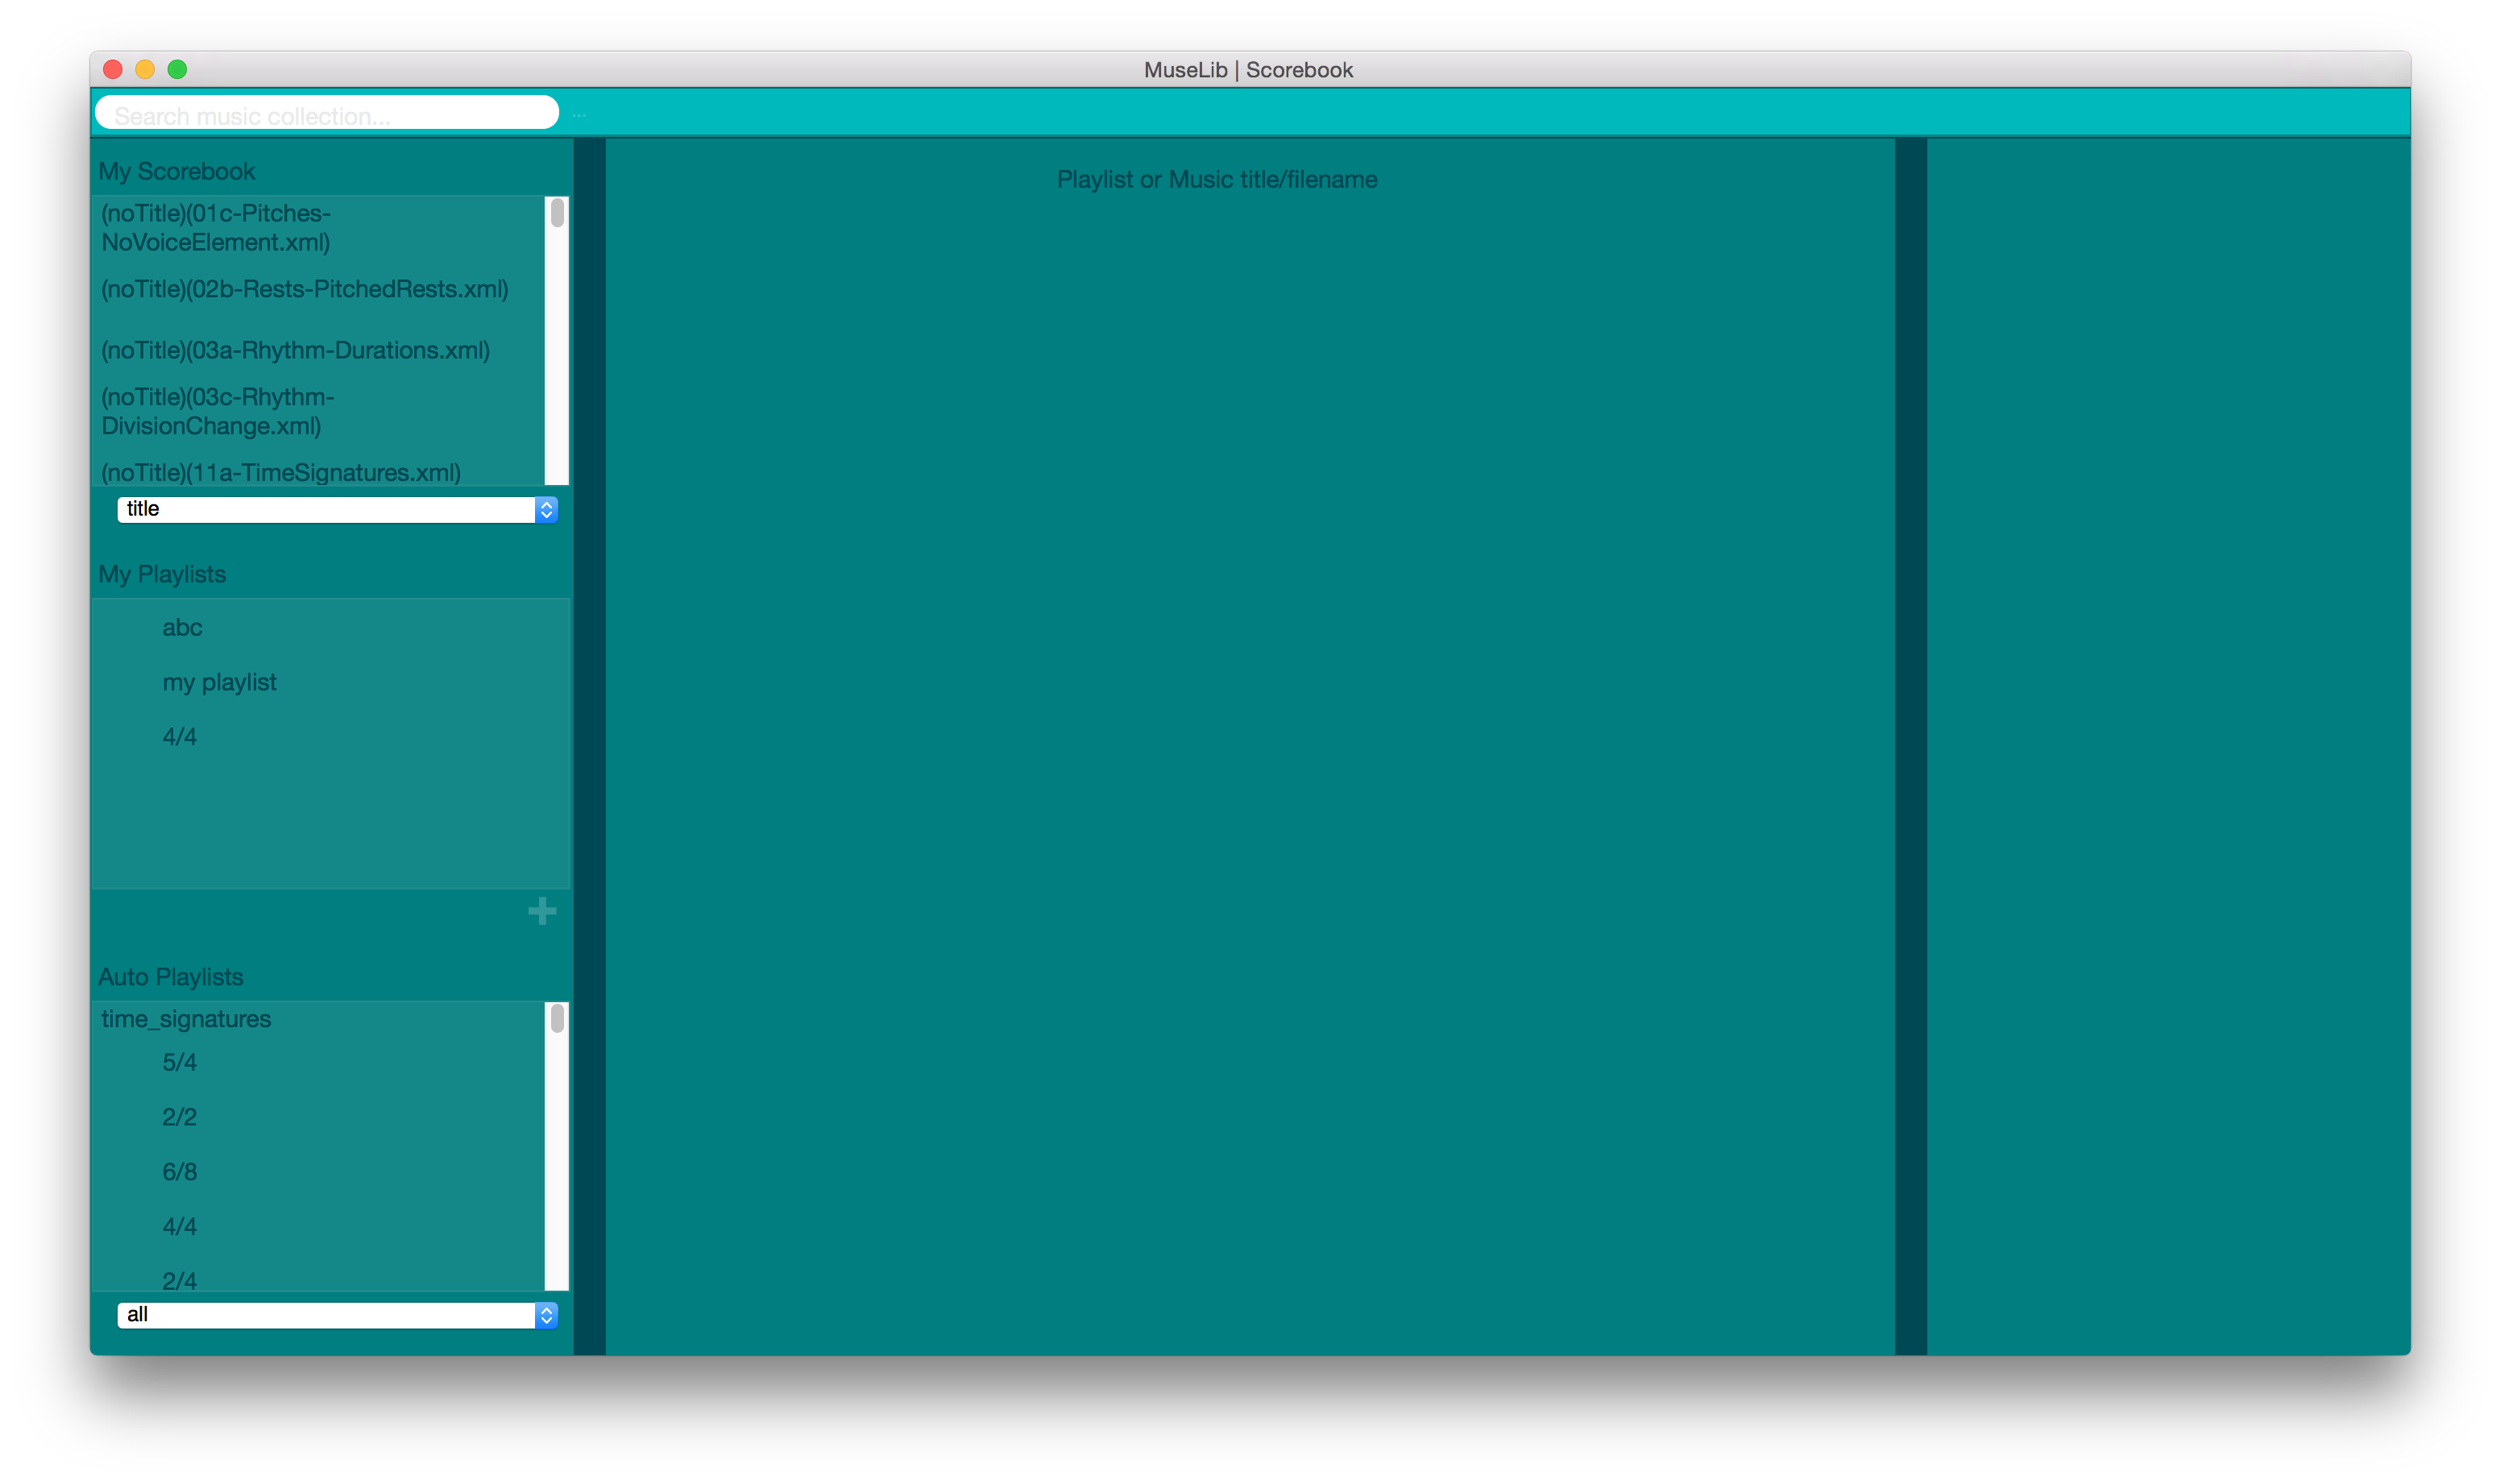
\includegraphics[width=400pt]{teal}
\caption{The teal theme}
\label{fig:theme4}	
\end{figure}

\subsubsection{Customising your widget views}
Any and all of the widgets to the right and left of the main pane can be hidden or displayed using the View menu, as shown in figure \ref{fig:view}.

\begin{figure}[H]
\centering
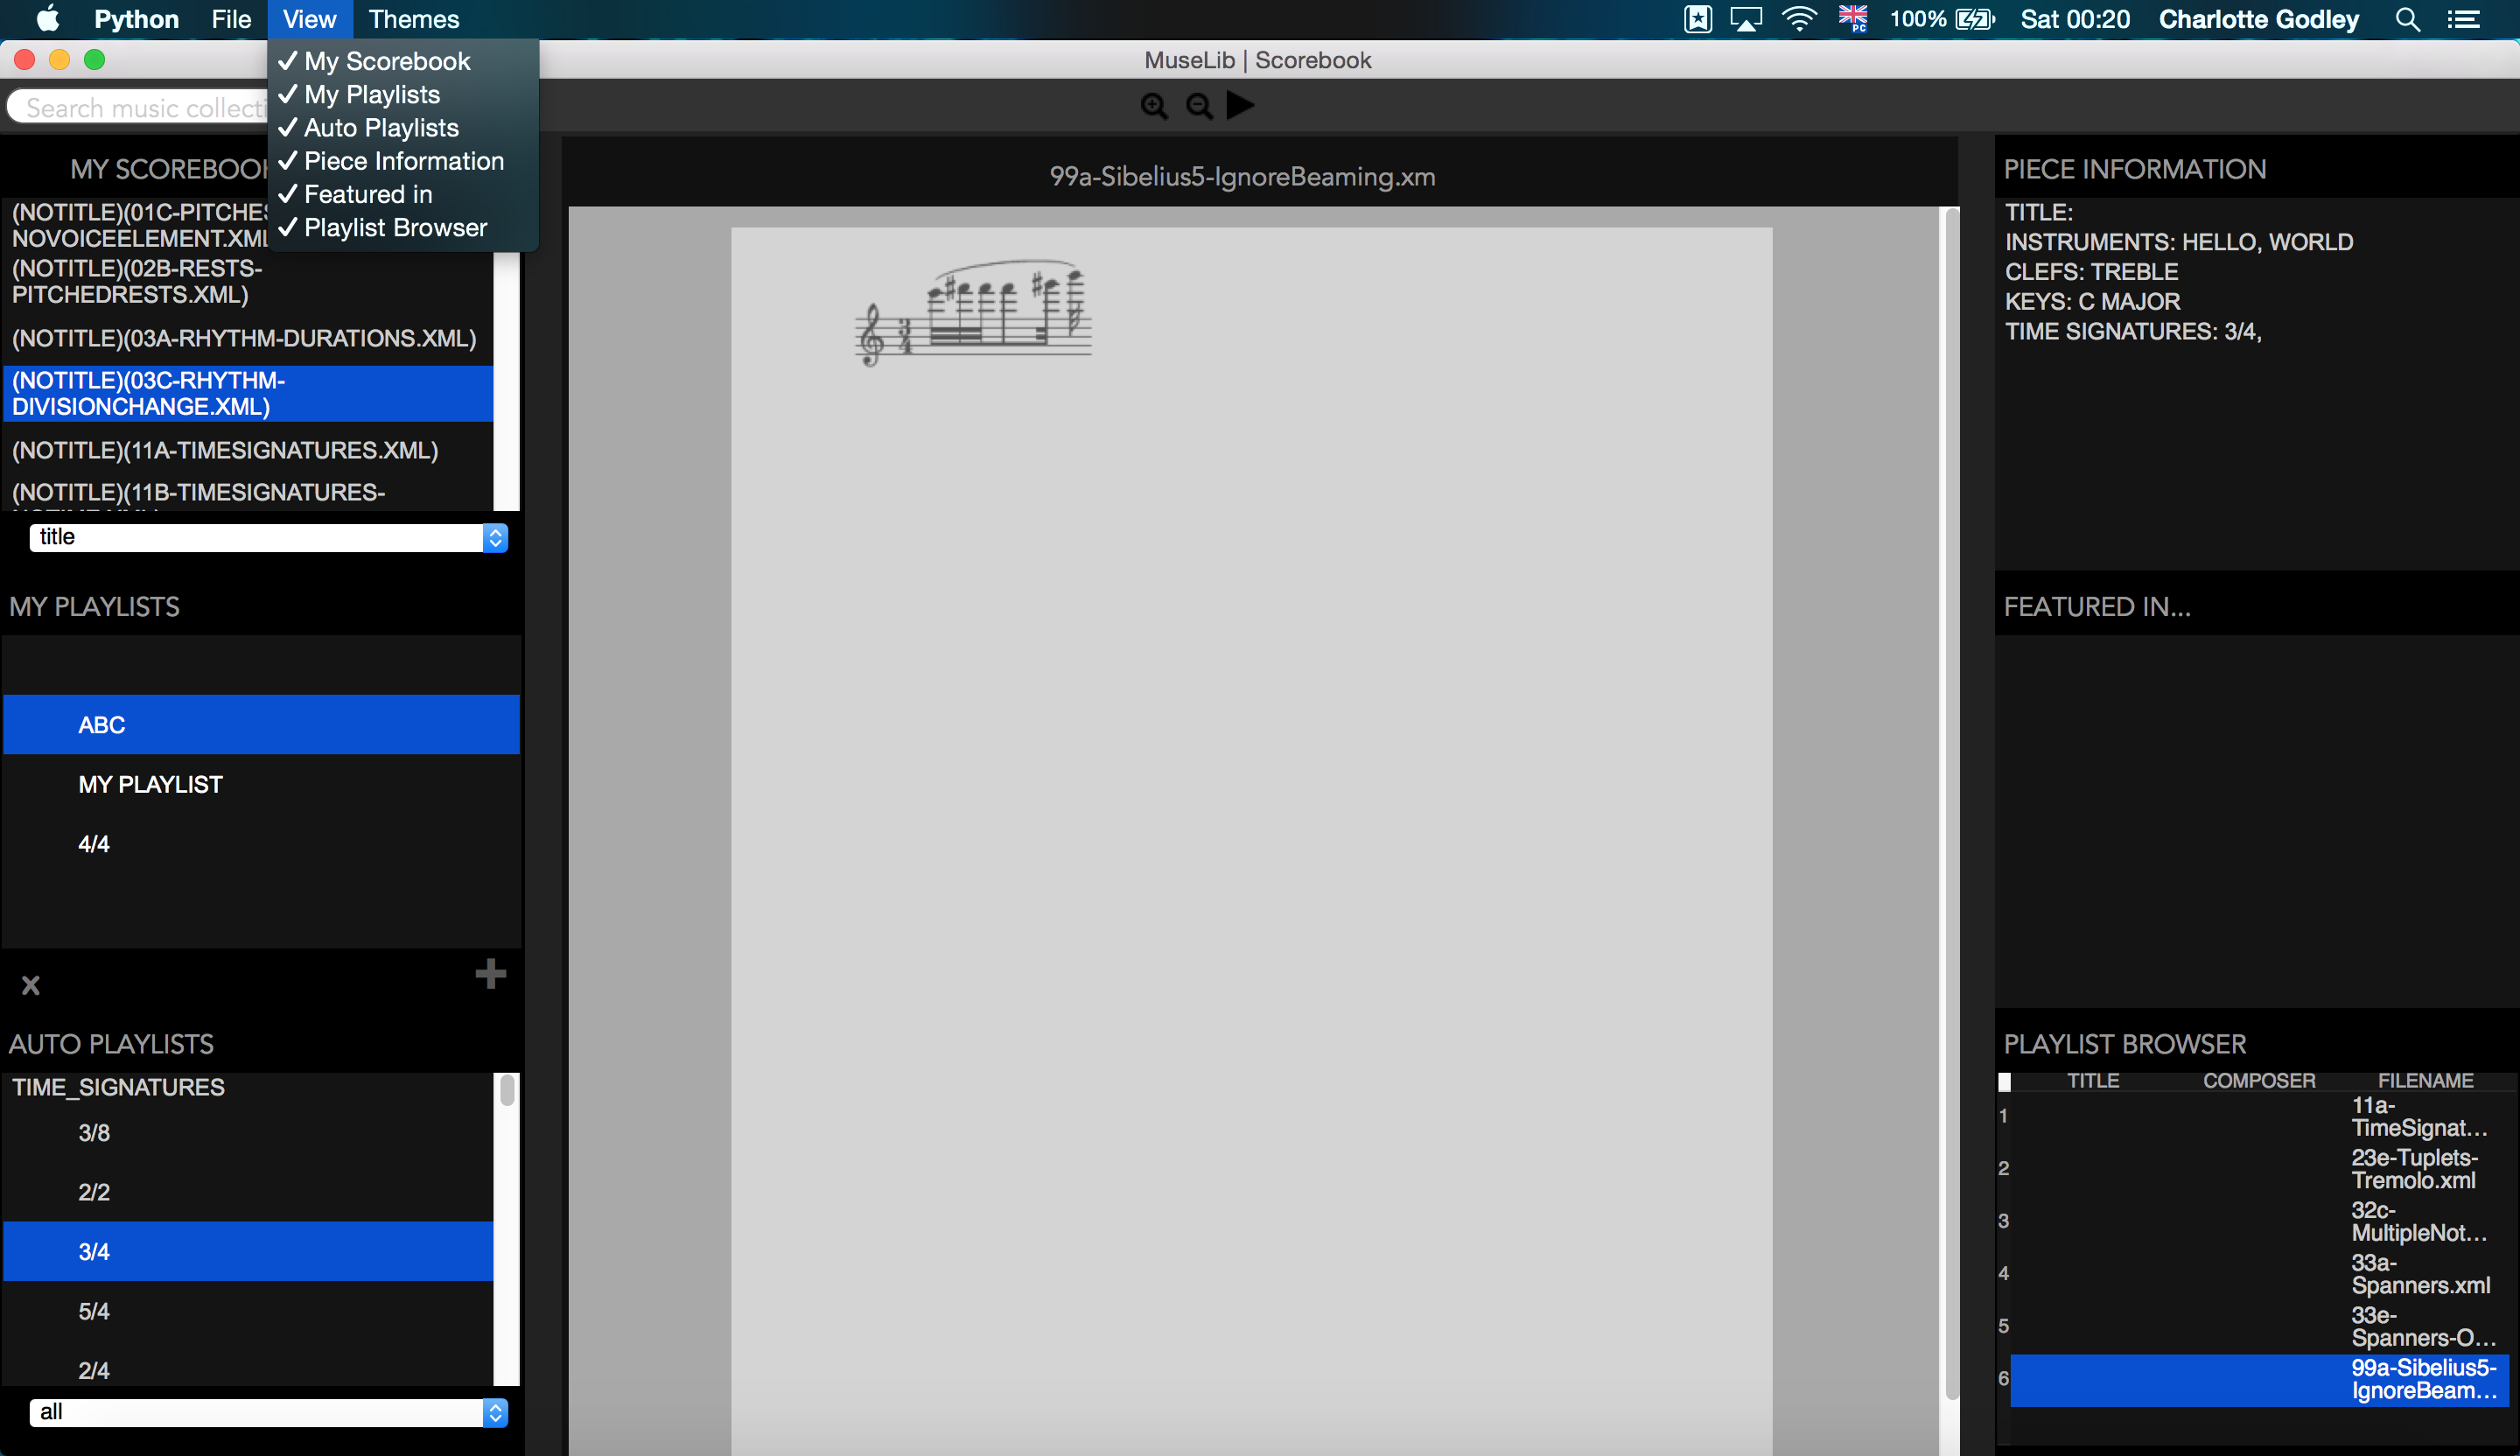
\includegraphics[width=500pt]{view}
\caption{The view menu}
\label{fig:view}	
\end{figure}



\end{document}
